\providecommand{\toplevelprefix}{../..}  % necessary for subfile bibliography + figures compilation to work, do not move this after documentclass
\documentclass[../../book-main.tex]{subfiles}

\begin{document}

\chapter{Entropy, Diffusion, Denoising, and Lossy Coding}\label{app:entropy}\label{app:diffusion-denoising}

\begin{quote}
``{\em The increase of disorder or entropy with time is one example of what is called an arrow of time, something that distinguishes the past from the future, giving a direction to time.}''

$~$\hfill -- A Brief History of Time, Stephen Hawking
 \end{quote}
\vspace{5mm}

In this appendix we provide proofs for several facts, mentioned in
\Cref{ch:general-distribution}, which are related to differential entropy, how
it evolves under diffusion processes, and its connections to lossy coding. We
will make the following mild assumption about the random variable representing
the data source, denoted \(\vx\).

\begin{assumption}\label{assumption:entropy_x_compact_support}
    \(\vx\) is supported on a compact set \(\cS \subseteq \R^{D}\) of radius at most \(R\), i.e., \(R \doteq \sup_{\vxi \in \cS}\norm{\vxi}_{2}\).
\end{assumption}

In particular, since compact sets in Euclidean space are bounded, it holds \(R < \infty\). We will consistently use the notation \(B_{r}(\vxi) \doteq \{\vu \in \R^{D} \colon \norm{\vxi - \vu}_{2} \leq r\}\) to denote the Euclidean ball of radius \(r\) centered at \(\vxi\). In this sense, \Cref{assumption:entropy_x_compact_support} has \(\cS \subseteq B_{R}(\vzero)\).

Notice that this assumption holds for (almost) all variables we care about in practice, as it is (often) imposed by a normalization step during data pre-processing. 

\section{Differential Entropy of Low-Dimensional Distributions}\label{sec:low_dim_entropy}

In this short appendix we provide a proof of the following fact.

\begin{theorem}\label{thm:degenerate_entropy_negative_infinity}
    Let \(\vx\) be any random variable such that \Cref{assumption:entropy_x_compact_support} holds, and the support \(\cS\) of \(\vx\) has \(0\) volume.\footnote{Formally this means that \(\cS\) is Borel measurable with Borel measure \(0\).} Then \(h(\vx) = -\infty\).
\end{theorem}
\begin{proof}
    We will show this for the case that \(\vx\) is uniform on \(\cS\); this setting captures the essential ideas without being too technical. The basic idea is to take an \(\eps\)-thickening of \(\cS\), say \(\cS_{\eps}\) defined as 
    \begin{equation}
        S_{\eps} = \bigcup_{\vxi \in \cS}B_{\eps}(\vxi)
    \end{equation}
    and visualized in \Cref{fig:entropy_eps_thickening}.
    \begin{figure}[th]
        \centering
        \begin{tikzpicture}
            \def\radius{0.2cm} % Define epsilon value
            \def\curve{(0,0) .. controls (1,1.5) and (3,-0.5) .. (4,1)} % Define the curve S

            % Draw many overlapping circles along the curve to represent the thickening S_eps
            % Use a decoration to place marks (circles) along the path
            \path[decoration={markings, mark=between positions 0 and 1 step 0.02 with {
                    % Fill a circle at each mark; low opacity to show overlap
                    \fill[red!30, opacity=0.5, draw=none] (0,0) circle (\radius);
                }}, postaction={decorate}] \curve;

            % Draw the original curve S on top, thicker and in blue
            \draw[blue, thick] \curve node[right, blue] {$\cS$};

            % Choose an example point x on the curve S
            \coordinate (p_on_curve) at (2, 0.5); % Approximate point on the curve
            % Draw the specific ball B_eps(x) for this x, slightly darker/more opaque
            \fill[red!50, opacity=0.7] (p_on_curve) circle (\radius);
            % Mark the point x
            \fill[black] (p_on_curve) circle (1pt) node[below left] {$x$};
            % Add an arrow indicating the radius epsilon for this specific ball

            % Label the thickened region S_eps, placing the label appropriately
             \node[red, below right] at (3.5, -0.2) {$\cS_{\eps} = \bigcup_{\vxi \in S} B_{\eps}(\vxi)$};

        \end{tikzpicture}
        \caption{Illustration of the \(\eps\)-thickening \(\cS_\eps\) of a curve \(\cS \subseteq \R^{2}\).}
        \label{fig:entropy_eps_thickening}
    \end{figure}
    We will work with random variables whose support is \(\cS_{\eps}\), which is fully-dimensional, and take the limit as \(\eps \to 0\).

    Thus let \(\vx \sim \dUnif(\cS)\) such that it does not have a density\footnote{w.r.t.~the Borel measure on \(\R^{D}\).} and \(\vx_{\eps} \sim \dUnif(\cS_{\eps})\). Since \(\cS_{\eps}\) has positive volume, \(\vx_{\eps}\) has a density \(p_{\eps}\) equal to
    \begin{equation}
        p_{\eps}(\vxi) = \indvar(\vxi \in \cS_{\eps}) \cdot \frac{1}{\volume(\cS_{\eps})}.
    \end{equation}
    Since \(\vx\) does not have a density, the way to make sense of \(h(\vx)\) is through the equality 
    \begin{equation}
        h(\vx) = \lim_{\eps \searrow 0}h(\vx_{\eps});
    \end{equation}
    we will show that the latter limit evaluates to \(-\infty\).

    Indeed, using the convention that \(0 \log 0 = 0\), it holds
    \begin{align}
        h(\vx_{\eps}) 
        &= -\int_{\R^{D}}p_{\eps}(x)\log p_{\eps}(x)\odif{x} \\ 
        &= -\int_{\cS_{\eps}}\frac{1}{\volume(\cS_{\eps})} \log\rp{\frac{1}{\volume(\cS_{\eps})}}\odif{\vxi} \\ 
        &= \frac{\log(\volume(\cS_{\eps}))}{\volume(\cS_{\eps})}\int_{\cS_{\eps}}\odif{\vxi} \\ 
        &= \log(\volume(\cS_{\eps})).
    \end{align}
    Since \(\cS\) is compact \(\volume(\cS_{\eps})\) is finite and tends to \(0\) as \(\eps \searrow 0\).\footnote{In the case where \(\cS\) is not compact and \(\vx\) is not uniform on \(\cS\), we define a more refined version of \(\vx_{\eps}\) whose density at \(\vxi\) changes at different rates in the directions orthogonal to and aligned with \(\cS\) at \(\vxi\). This density results in a different calculation which does not involve the volume of \(\cS_{\eps}\) but rather something like the effective volume taken up by \(\vx_{\eps}\), which is finite and vanishing as \(\eps \searrow 0\).} Thus
    \begin{equation}
        h(\vx) = \lim_{\eps \searrow 0}h(\vx_{\eps}) = \lim_{\eps \searrow 0}\log(\volume(\cS_{\eps})) = -\infty,
    \end{equation}
    as desired.
\end{proof}

The above theorem is actually a corollary of a much more famous and celebrated set of results about the maximum possible entropy of \(\vx\) subject to certain constraints on the distribution of \(\vx\). We would be remiss to not provide the results here, but we do not give the proofs; a suitable reference would be \cite{poliyanski2024information}.
\begin{theorem}\label{thmx:max_entropy}
    Let \(\vx\) be a random variable on \(\R^{D}\).
    \begin{enumerate}
        \item If \(\vx\) is supported on a compact set \(\cS \subseteq \R^{D}\) (i.e., \Cref{assumption:entropy_x_compact_support}) then
        \begin{equation}
            h(\vx) \leq h(\dUnif(\cS)) = \log \volume(\cS).
        \end{equation}
        \item If \(\vx\) has finite covariance such that, for a PSD matrix \(\vSigma \in \PSD(D)\), it holds \(\Cov(\vx) \preceq \vSigma\) (w.r.t.~the PSD ordering, i.e., \(\vSigma - \Cov(\vx)\) is PSD), then
        \begin{equation}
            h(\vx) \leq h(\dNorm(\vzero, \vSigma)) = \frac{1}{2}\log((2\pi e)^{D}\det\vSigma).
        \end{equation}
        \item If \(\vx\) has finite second moment such that, for a constant \(a \geq 0\), it holds \(\Ex\norm{\vx}_{2}^{2} \leq a\), then
        \begin{equation}
            h(\vx) \leq h\rp{\dNorm\rp{\vzero, \frac{a}{D}\vI}} = \frac{D}{2}\log\frac{2\pi e a}{D}.
        \end{equation}
    \end{enumerate}
\end{theorem}
Clearly \Cref{thm:degenerate_entropy_negative_infinity} is a special case of \Cref{thmx:max_entropy}.1 with \(\volume(\cS) = 0\).



\section{Diffusion and Denoising Processes}\label{sec:entropy_diffusion}

In the main body (\Cref{ch:general-distribution}), we considered a random variable \(\vx\), and a stochastic process defined by \eqref{eq:additive_gaussian_noise_model}, i.e.,
\begin{equation}\label{eq:app_additive_gaussian_noise_model}
    \vx_{t} = \vx + t\vg, \qquad  \forall t \in [0, T]
\end{equation}
where \(\vg \sim \dNorm(\vzero, \vI)\) independently of \(\vx\). 

The structure of this section is as follows. In \Cref{sub:diffusion_entropy_increases} we provide a formal theorem and crisp proof which shows that under \Cref{eq:app_additive_gaussian_noise_model} the entropy increases, i.e., \(\odv*{h(\vx_{t})}{t} > 0\). In \Cref{sub:denoising_entropy_decreases} we provide a formal theorem and crisp proof which shows that under \Cref{eq:app_additive_gaussian_noise_model}, the entropy decreases during denoising, i.e., \(h(\Ex[\vx_{s} \given \vx_{t}]) < h(\vx_{t})\) for all \(s < t\). In \Cref{sub:app_diffusion_intermediate_results} we provide proofs for technical lemmas that are needed to establish the claims in the previous subsections.

Before we start, we introduce some key notations. First, let \(\phi_{t}\) be the density of \(\dNorm(\vzero, t^{2}\vI)\), i.e.,
\begin{equation}\label{eq:gaussian_noise_time_t}
    \phi_{t}(\vxi) \doteq \frac{1}{(2\pi)^{D/2}t^{D}}\exp\rp{-\frac{\norm{\vxi}_{2}^{2}}{t^{2}}}.
\end{equation}
Next, \(\vx_{t}\) is supported on all of \(\R^{D}\), so it has a \textit{density}, which we denote \(p_{t}\) (as in the main body). A quick calculation shows that
\begin{equation}\label{eq:p_t_representation}
    p_{t}(\vxi) = \Ex[\phi_{t}(\vxi - \vx)],
\end{equation}
and from this representation it is possible to deduce (i.e., from \Cref{prop:diff_convolution}) that \(p_{t}\) is smooth (i.e., infinitely differentiable) in \(\vxi\), also smooth in \(t\), and positive everywhere. This fact is somewhat remarkable at first sight: even for a completely irregular random variable \(\vx\) (say, a Bernoulli random variable, which does not have a density), its Gaussian smoothing admits a density for every (arbitrarily small) \(t > 0\). The proof is left as an exercise for readers well-versed in mathematical analysis.

However, we also need to add an assumption about the \textit{smoothness} of the distribution of \(\vx\), which will eliminate some technical problems that occur around \(t = 0\) with low-dimensional distributions.\footnote{As then various quantities become highly irregular and dealing with them would require significant additional analysis.} Despite this, we expect that our results hold under milder assumptions with additional work. For now, let us assume:
\begin{assumption}\label{assumption:entropy_x_density}
    \(\vx\) has a twice continuously differentiable density, denoted \(p\).
\end{assumption}


\subsection{Diffusion Process Increases Entropy Over Time}\label{sub:diffusion_entropy_increases}

In this section appendix we provide a proof of \Cref{thm:diffusion_entropy_increases}. For convenience, we restate it as follows. 

\begin{theorem}[Diffusion Increases Entropy]\label{thm:diffusion_entropy_increases}
    Let \(\vx\) be any random variable such that \Cref{assumption:entropy_x_compact_support,assumption:entropy_x_density} hold, and let \((\vx_{t})_{t \in [0, T]}\) be the stochastic process \eqref{eq:app_additive_gaussian_noise_model}. Then 
    \begin{equation}\label{eq:diffusion_entropy_increases}
        h(\vx_{s}) < h(\vx_{t}), \qquad \forall s, t \colon 0 \leq s < t \leq T.
    \end{equation}
\end{theorem}
\begin{proof}
    Before we start, let us address a pedantic question: when does the inequality in \eqref{eq:diffusion_entropy_increases} make sense? We will show in \Cref{lem:diffusion_entropy_exists} that under our assumptions, the differential entropy is well-defined, is never \(+\infty\), and for \(t > 0\) is finite, so the (strict) inequality in \eqref{eq:diffusion_entropy_increases} makes sense.

    Pedantry aside, the crux of this proof is to show that the density \(p_{t}\) of \(\vx_{t}\) satisfies a particular partial differential equation, which is very similar to the \textit{heat equation}. The heat equation is a famous PDE which describes the diffusion of heat through space. This intuitively should make sense, and paints a mental picture: as the time \(t\) increases, the probability from the original (perhaps tightly concentrated) \(\vx\) disperses across all of \(\R^{D}\) like heat radiating from a source in a vacuum.
    
    Such PDEs for \(p_{t}\), known as \textit{Fokker-Planck equations} for more general stochastic processes, are very powerful tools, as they allow us to describe the instantaneous temporal derivatives of \(p_{t}\) in terms of the instantaneous spatial derivatives of \(p_{t}\), and vice versa, providing a concise description of the regularity and dynamics of \(p_{t}\). Once we obtain dynamics for \(p_{t}\), we can then use the system to obtain another one which describes the dynamics of \(h(\vx_{t})\), which after all is just a functional of \(p_{t}\).  

    The description of the PDE involves a mathematical object called the Laplacian \(\Delta\). Recall from your multivariable calculus class that the Laplacian operating on a differentiable-in-time and twice-differentiable-in-space function \(f \colon (0, T) \times \R^{D} \to \R\) is given by
    \begin{equation}
        \Delta f_{t}(\vxi) = \tr(\nabla^{2}f_{t}(\vxi)) = \sum_{i = 1}^{D}\pdv[order=2]{f_{t}}{\xi_{i}}(\vxi).
    \end{equation}
    
    Namely, from using the integral representation of \(p_{t}\) and differentiating under the integral, we can compute the derivatives of \(p_{t}\) (which we do in \Cref{prop:p_t_derivatives}) and observe that \(p_{t}\) satisfies the heat-like PDE
    \begin{equation}
        \pdv{p_{t}}{t}(\vxi) = t\Delta p_{t}(\vxi).
    \end{equation}
    Then for finding the dynamics of \(h(\vx_{t})\), we can use \Cref{prop:dutis} again as well as the heat-like PDE to get
    \begin{align}
        \odv*{h(\vx_{t})}{t}
        &= -\odv*{\int_{\R^{D}}p_{t}(\vxi)\log p_{t}(\vxi)\odif{\vxi}}{t} \\
        &= -\int_{\R^{D}}\pdv*{\bs{p_{t}(\vxi)\log p_{t}(\vxi)}}{t}\odif{\vxi} \\
        &= -\int_{\R^{D}}\pdv{p_{t}}{t}(\vxi)[1 + \log p_{t}(\vxi)]\odif{\vxi} \\
        &= -t\int_{\R^{D}}\Delta p_{t}(\vxi)[1 + \log p_{t}(\vxi)]\odif{\vxi}.
    \end{align}
    By using a slightly involved integration by parts argument (\Cref{lem:diffusion_ibp}), we obtain 
    \begin{align}
        \odv*{h(\vx_{t})}{t}
        &= t\int_{\R^{D}}\ip{\nabla \log p_{t}(\vxi)}{\nabla p_{t}(\vxi)}\odif{\vxi} \\
        &= t\int_{\R^{D}}\frac{\norm{\nabla p_{t}(\vxi)}_{2}^{2}}{p_{t}(\vxi)}\odif{\vxi} \\
        &> 0
    \end{align}
    where strict inequality holds in the last line because, for it to not hold, \(\nabla p_{t}(\vxi)\) would need to vanish almost everywhere (i.e., everywhere except possibly on a set of zero volume), but this would imply that \(p_{t}\) would be constant almost everywhere, a contradiction with a fact that \(p_{t}\) is a density.

    To complete the proof we just use the fundamental theorem of calculus
    \begin{equation}
        h(\vx_{t}) = h(\vx_{s}) + \int_{s}^{t}\odv*{h(\vx_{u})}{u}\odif{u} > h(\vx_{s}),
    \end{equation}
    which proves the claim. (Note that this does not make sense when \(h(\vx_{s}) = -\infty\), which can only happen when \(s = 0\) and \(h(\vx) = -\infty\), but in this case \(h(\vx_{t}) > -\infty\) so the claim is vacuously true anyways.)
\end{proof}

\subsection{Denoising Process Reduces Entropy Over Time}\label{sub:denoising_entropy_decreases}

Recall that in \Cref{sub:intro_diffusion_denoising} we start with the random variable \(\vx_{T}\) and iteratively denoise it using iterations of the form
\begin{equation}\label{eq:app_denoising_iteration}
    \hat{\vx}_{s} \doteq \Ex[\vx_{s} \mid \vx_{t} = \hat{\vx}_{t}] = \frac{s}{t}\hat{\vx}_{t} + \bp{1 - \frac{s}{t}}\bar{\vx}^{\ast}(t, \hat{\vx}_{t}).
\end{equation}
for \(s, t \in \{t_{0}, t_{1}, \dots, t_{L}\}\) with \(s < t\) and \(\vx_{T} = \hat{\vx}_{T}\). We wish to prove that \(h(\hat{\vx}_{s}) < h(\hat{\vx}_{t})\), showing that the denoising process actually reduces the entropy.

Before we go about doing this, we make several remarks about the problem statement. First, Tweedie's formula \eqref{eq:tweedie} says that 
\begin{equation}
    \bar{\vx}^{\ast}(t, \vx_{t}) = \vx_{t} + t^{2}\nabla p_{t}(\vx_{t}),
\end{equation}
which likens a full denoising step from time \(t\) to time \(0\) to a gradient step on the log-density of \(\vx_{t}\). Can we get a similar result for the full denoising step from time \(t\) to time \(s\) in \eqref{eq:app_denoising_iteration}? It turns out that indeed we can, and it is pretty simple. By using \eqref{eq:app_denoising_iteration} and Tweedie's formula \eqref{eq:tweedie}, we obtain
\begin{equation}\label{eq:app_denoising_iteration_score}
    \Ex[\vx_{s} \mid \vx_{t}] = \frac{s}{t}\vx_{t} + \bp{1 - \frac{s}{t}}\bp{\vx_{t} + t^{2}\nabla_{\vx_{t}}\log p_{t}(\vx_{t})} = \vx_{t} + \bp{1 - \frac{s}{t}}t^{2}\nabla_{\vx_{t}}\log p_{t}(\vx_{t}).
\end{equation}
So this iterative denoising step is again a gradient step on the perturbed log-density \(\log p_{t}\) with a shrunken step size. In particular, this step can be seen as a perturbation of the distribution of the random variable \(\vx_{t}\) by the \textit{score function vector field}, suggesting a connection to stochastic differential equations (SDEs) and the theory of diffusion models \cite{song2020score}. Indeed, a proof of the following result \Cref{thm:conditioning_reduces_entropy} can be developed using this powerful machinery and a limiting argument (e.g., following the technical approach in the exposition of \cite{DBLP:conf/iclr/ChenC0LSZ23}). We will give a simpler proof here, which will use only elementary tools and  thereby illuminate some of the key quantities behind the process of entropy reduction via denoising. On the other hand, we will need to deal with some slightly technical calculations due to the fact that the denoising process in \Cref{thm:conditioning_reduces_entropy} does \textit{not} correspond exactly to the \textit{reverse} process associated to the noise addition process that generates the observation \(\vx_{t}\).\footnote{For those familiar with diffusion models, we refer here to the time-reversed forward process not coinciding with the sequence of iterates generated by the process defined by \Cref{thm:conditioning_reduces_entropy}. These processes coincide in a certain limit where infinitely many steps of \Cref{thm:conditioning_reduces_entropy} are taken with infinitely small levels of noise added at each step; for general, finite steps, we must introduce some approximations regardless of the level of sophistication of our tools.}

We want to prove that \(h(\Ex[\vx_{s} \mid \vx_{t}]) < h(\vx_{t})\), i.e., formally:
\begin{theorem}\label{thm:conditioning_reduces_entropy}
    Let \(\vx\) be any random variable such that \Cref{assumption:entropy_x_compact_support,assumption:entropy_x_density} hold, and let \((\vx_{t})_{t \in [0, T]}\) be the stochastic process \eqref{eq:app_additive_gaussian_noise_model}. Then 
    \begin{equation}
        h(\Ex[\vx_{s} \mid \vx_{t}]) < h(\vx_{t}), \qquad \forall s, t \in [0, T] \colon \quad 0 < t \leq \frac{R}{\sqrt{2D}}, \quad 0 \leq s  < t\cdot\min\bc{1, \frac{R^{2}/D - 2t^{2}}{R^{2}/D - t^{2}}}.
    \end{equation}
\end{theorem}
\begin{proof}
    This proof uses two main ideas:
    \begin{enumerate}
        \item First, write down a density for \(\Ex[\vx_{s} \mid \vx_{t}]\) using a change-of-variables formula.
        \item Second, bound this density to control the entropy.
    \end{enumerate}
    The change of variables is justified by \Cref{cor:gribonval_A2}, which was originally derived in \cite{Gribonval2011-pf}.

    We execute these ideas now. From \Cref{cor:gribonval_A2}, we obtain that the function \(\bar{\vx}\) defined as \(\bar{\vx}(\vxi) \doteq \Ex[\vx_{s} \given \vx_{t} = \vxi]\) is differentiable, injective, and thus invertible on its range, which we henceforth denote \(\cX \subseteq \R^{D}\). We denote its inverse as \(\bar{\vx}^{-1}\). Using a change-of-variables formula, the density \(\bar{p}\) of \(\bar{\vx}(\vx_{t})\) is given by 
    \begin{equation}
        \bar{p}(\vxi) \doteq \frac{(p_{t} \circ \bar{\vx}^{-1})(\vxi)}{\det(\bar{\vx}^{\prime}(\bar{\vx}^{-1}(\vxi)))},
    \end{equation}
    where (recall, from \Cref{app:optimization}) \(\bar{\vx}^{\prime}\) is the Jacobian of \(\bar{\vx}\). Since from \Cref{lem:gribonval_A1} we know \(\bar{\vx}^{\prime}\) is a positive definite matrix, the determinant is positive and so the whole density is positive. Then it follows that 
    \begin{align}
        h(\bar{\vx}(\vx_{t}))
        &= -\int_{\cX}\frac{(p_{t} \circ \bar{\vx}^{-1})(\vxi)}{\det(\bar{\vx}^{\prime}(\bar{\vx}^{-1}(\vxi)))} \log \frac{(p_{t} \circ \bar{\vx}^{-1})(\vxi)}{\det(\bar{\vx}^{\prime}(\bar{\vx}^{-1}(\vxi)))} \odif{\vxi} \\ 
        &= -\int_{\cX}\frac{(p_{t} \circ \bar{\vx}^{-1})(\vxi)}{\det(\bar{\vx}^{\prime}(\bar{\vx}^{-1}(\vxi)))} \log((p_{t} \circ \bar{\vx}^{-1})(\vxi))\odif{\vxi} \\ 
        &\qquad + \int_{\cX}\frac{(p_{t} \circ
        \bar{\vx}^{-1})(\vxi)}{\det(\bar{\vx}^{\prime}(\bar{\vx}^{-1}(\vxi)))}\log\det\rp{\bar{\vx}^{\prime}(\bar{\vx}^{-1}(\vxi))}\odif{\vxi} \\ 
        &= -\int_{\R^{D}}p_{t}(\vxi)\log p_{t}(\vxi)\odif{\vxi}
        + \int_{\cX}\frac{(p_{t} \circ
        \bar{\vx}^{-1})(\vxi)}{\det(\bar{\vx}^{\prime}(\bar{\vx}^{-1}(\vxi)))}\log\det\rp{\bar{\vx}^{\prime}(\bar{\vx}^{-1}(\vxi))}\odif{\vxi} \\ 
        &= h(\vx_{t}) - \int_{\cX}\frac{(p_{t} \circ \bar{\vx}^{-1})(\vxi)}{\det(\bar{\vx}^{\prime}(\bar{\vx}^{-1}(\vxi)))}\log\rp{\frac{1}{\det(\bar{\vx}^{\prime}(\bar{\vx}^{-1}(\vxi)))}}\odif{\vxi}.
    \end{align}
    We will study the last term (including the \(-\)), and show that it is negative.

    By concavity, one has \(-x\log x \leq 1 - x\) for every \(x \geq 0\). Hence 
    \begin{align}
        h(\bar{\vx}(\vx_{t})) - h(\vx_{t})
        &= - \int_{\cX}\frac{(p_{t} \circ \bar{\vx}^{-1})(\vxi)}{\det(\bar{\vx}^{\prime}(\bar{\vx}^{-1}(\vxi)))}\log\rp{\frac{1}{\det(\bar{\vx}^{\prime}(\bar{\vx}^{-1}(\vxi)))}}\odif{\vxi} \\ 
        &\leq  \int_{\cX}(p_{t} \circ \bar{\vx}^{-1})(\vxi)\cdot \bp{1 - \frac{1}{\det(\bar{\vx}^{\prime}(\bar{\vx}^{-1}(\vxi)))}}\odif{\vxi} \\ 
        &= \int_{\cX}(p_{t} \circ \bar{\vx}^{-1})(\vxi)\odif{\vxi} - \int_{\cX}\frac{(p_{t} \circ \bar{\vx}^{-1})(\vxi)}{\det(\bar{\vx}^{\prime}(\bar{\vx}^{-1}(\vxi)))}\odif{\vxi} \\
        &= \int_{\R^{D}}p_{t}(\vxi)\det\rp{\bar{\vx}^{\prime}(\bar{\vx}^{-1}(\vxi))}\odif{\vxi} - \int_{\cX}\bar{p}(\vxi)\odif{\vxi} \\
        &= \int_{\R^{D}}p_{t}(\vxi)\det\rp{\vI + \bp{1 - \frac{s}{t}}t^{2}\nabla^{2}\log p_{t}(\vxi)}\odif{\vxi} - 1.
    \end{align}
    Now, by the AM-GM inequality on eigenvalues, we have for any symmetric positive definite matrix \(\vM \in \PSD(D)\) the bound 
    \begin{equation}
        \det(\vM)^{1/D} = \prod_{i = 1}^{D}\lambda_{i}(\vM)^{1/D} \leq \frac{\sum_{i = 1}^{D}\lambda_{i}(\vM)}{D} = \frac{\tr(\vM)}{D},
    \end{equation}
    which we can apply to the above expression and obtain 
    \begin{align}
        &\int_{\R^{D}}p_{t}(\vxi)\det\rp{\vI + \bp{1 - \frac{s}{t}}t^{2}\nabla^{2}\log p_{t}(\vxi)}\odif{\vxi} \\
        &\leq \int_{\R^{D}} p_{t}(\vxi) \tr\rp{\frac{1}{D}\bs{\vI + \bp{1 - \frac{s}{t}}t^{2}\nabla^{2}\log p_{t}(\vxi)}}^{D}\odif{\vxi} \\
        &= \int_{\R^{D}} p_{t}(\vxi)\bp{1 + \frac{\bp{1 - \frac{s}{t}}t^{2}}{D}\tr(\nabla^{2}\log p_{t}(\vxi))}^{D}\odif{\vxi} \\
        &= \int_{\R^{D}} p_{t}(\vxi)\bp{1 + \frac{\bp{1 - \frac{s}{t}}t^{2}}{D}\Delta \log p_{t}(\vxi)}^{D}\odif{\vxi}.
    \end{align}
    From \Cref{lem:app_diffusion_laplacian_control}, it holds (where, recall, \(R\) is the radius of the support of \(\vx\) as in \Cref{assumption:entropy_x_compact_support})
    \begin{equation}
        \abs{\Delta \log p_{t}(\vxi)} \leq \max\rp{\frac{D}{t^{2}}, \abs*{\frac{R^{2}}{t^{4}} - \frac{D}{t^{2}}}} =: U_{t}.
    \end{equation}
    Then it holds
    \begin{equation}
        -\frac{\bp{1 - \frac{s}{t}}t^{2}}{D}U_{t} \leq \frac{\bp{1 - \frac{s}{t}}t^{2}}{D}\Delta \log p_{t}(\vxi) \leq \frac{\bp{1 - \frac{s}{t}}t^{2}}{D}U_{t}.
    \end{equation}
    Meanwhile, the function \(x \mapsto (1 + x)^{D}\) is convex on \([-1, \infty)\), so for
    \(-(1-s/t)t^{2}U_{t}/D \leq x \leq (1-s/t)t^{2}U_{t}/D\) we have 
    \begin{align}
        (1 + x)^{d} 
        &\leq \bp{1 - \frac{\bp{1 - \frac{s}{t}}t^{2}U_{t}}{D}}^{D} + \underbrace{\bs{\bp{1 + \frac{\bp{1 - \frac{s}{t}}t^{2}U_{t}}{D}}^{D} - \bp{1 - \frac{\bp{1 - \frac{s}{t}}t^{2}U_{t}}{D}}^{D}}}_{M(s, t, D)}x \\ 
        &\leq 1 + M(s, t, D)x.
    \end{align}
    Here \(M(s, t, D) > 0\) since \(U_{t} > 0\). In the above bound, we need to verify that the lower bound for \(x\) is \(\geq -1\). Indeed,
    \begin{align}
        -\frac{\bp{1 - \frac{s}{t}}t^{2}}{D}U_{t}
        &= -\frac{\bp{1 - \frac{s}{t}}t^{2}}{D}\max\rp{\frac{D}{t^{2}}, \abs*{\frac{R^{2}}{t^{4}} - \frac{D}{t^{2}}}} \\ 
        &= -\bp{1 - \frac{s}{t}}\max\rp{1, \abs*{\frac{R^{2}}{Dt^{2}} - 1}}
    \end{align}
    Notice that this is \(\geq -1\) if and only if \(\bp{1 - \frac{s}{t}}\cdot\bp{\frac{R^{2}}{Dt^{2}} - 1} \geq 1\), i.e., \(0 < t < R/\sqrt{2D}\) and \(0 \leq s \leq t\cdot\frac{R^{2}/D - 2t^{2}}{R^{2}/D - t^{2}}\), as granted by the assumptions.
    
    Applying this bound, we obtain
    \begin{align}
        &\int_{\R^{D}} p_{t}(\vxi)\bp{1 + \frac{\bp{1 - \frac{s}{t}}t^{2}}{D}\Delta \log p_{t}(\vxi)}^{D}\odif{\vxi} \\ 
        &\leq \int_{\R^{D}}p_{t}(\vxi)\bp{1 + M(s, t, D)\Delta \log p_{t}(\vxi)}\odif{\vxi} \\
        &= 1 + M(s, t, D)\int_{\R^{D}}p_{t}(\vxi)\Delta \log p_{t}(\vxi)\odif{\vxi} \\
        &= 1 - M(s, t, D)\int_{\R^{D}}\ip{\nabla p_{t}(\vxi)}{\nabla\log p_{t}(\vxi)}\odif{\vxi} \\
        &= 1 - M(s, t, D)\int_{\R^{D}}\frac{\norm{\nabla p_{t}(\vxi)}_{2}^{2}}{p_{t}(\vxi)}\odif{\vxi},
    \end{align}
    where the last few lines are the same as in the proof of \Cref{thm:diffusion_entropy_increases}. Combining this result with our previous estimate,
    \begin{equation}
        h(\bar{\vx}(\vx_{t})) - h(\vx_{t}) \leq - M(s, t, D)\int_{\R^{D}}\frac{\norm{\nabla p_{t}(\vxi)}_{2}^{2}}{p_{t}(\vxi)}\odif{\vxi} < 0
    \end{equation}
    where the inequality is strict by the same argument as in \Cref{thm:diffusion_entropy_increases}.
\end{proof}

Notice that the bounds for \(s\) and \(t\) depend on the radius \(R\) of the data distribution, and are not so general as the bounds in \Cref{thm:diffusion_entropy_increases}. The result is actually ``as general as needed'' in the following sense. Note that if \(\vx\) has a twice continuously differentiable density supported on the ball of radius \(R\) centered at \(\vzero\), then it does for \(2R\), and \(3R\), and so on, i.e., for any ball of radius \(R^{\prime} > R\). Thus one strategy to get the appropriate denoising guarantee is: fix a data dimension \(D\) and discretization schedule, and then set (in the analysis) the data radius \(R\) to be very large such that each denoising step satisfies the requirements for entropy decrease given in \Cref{thm:conditioning_reduces_entropy}. Then each step of the denoising process will indeed reduce the entropy, as desired.

 
\subsection{Technical Lemmas and Intermediate Results}\label{sub:app_diffusion_intermediate_results}

In this subsection we present technical results which power our main two conceptual theorems. Our presentation will be more or less standard for mathematics; we will start with the higher-level results first, and gradually move back to the more incremental results. The higher-level results will use the incremental results, and in this way we have an easy-to-read dependency ordering of the results: no result depends on those before it. Results which do not depend on each other are generally ordered by the place they appear in the above pair of proofs. 


\subsubsection{Finitneness of the Differential Entropy}

We first show that the entropy exists along the stochastic process and is finite.

\begin{lemma}\label{lem:diffusion_entropy_exists}
    Let \(\vx\) be any random variable, and let \((\vx_{t})_{t \in [0, T]}\) be the stochastic process \eqref{eq:app_additive_gaussian_noise_model}. 
    \begin{enumerate}
        \item For \(t > 0\), the differential entropy \(h(\vx_{t})\) exists and is \(> -\infty\).
        \item If in addition \Cref{assumption:entropy_x_compact_support} holds for \(\vx\), then \(h(\vx) < \infty\) and \(h(\vx_{t})\ < \infty\).
    \end{enumerate}
\end{lemma}
\begin{proof}
    To prove \Cref{lem:diffusion_entropy_exists}.1, we use a classic yet tedious analysis argument. Since \(\vx_{t}\) has a density, we can write 
    \begin{equation}
        h(\vx_{t}) = -\int_{\R^{D}}p_{t}(\vxi)\log p_{t}(\vxi) \odif{\vxi}.
    \end{equation}
    Accordingly, let \(g \colon \R^{D} \to \R\) be defined as 
    \begin{equation}
        g(\vxi) \doteq -p_{t}(\vxi)\log p_{t}(\vxi) \implies h(\vx_{t}) = \int_{\R^{D}}g(\vxi)\odif{\vxi}.
    \end{equation}
    As usual to bound the value of an integral in analysis, define 
    \begin{equation}
        g_{+}(\vxi) \doteq \max(g(\vxi), 0), \quad g_{-}(\vxi) \doteq \max(-g(\vxi), 0) \quad \implies \quad g = g_{+} - g_{-}\quad \text{and} \quad g_{+}, g_{-} \geq 0.
    \end{equation}
    Then 
    \begin{equation}
        h(\vx_{t}) = \int_{\R^{D}}g_{+}(\vxi)\odif{\vxi} - \int_{\R^{D}}g_{-}(\vxi)\odif{\vxi},
    \end{equation}
    and both integrals are guaranteed to be non-negative since their integrands are. 
    
    In order to show that \(h(\vx_{t})\) is well-defined, we need to show that \(\int_{\R^{D}}g_{+}(\vxi)\odif{\vxi} < \infty\) or \(\int_{\R^{D}}g_{-}(\vxi) \odif{\vxi} < \infty\). To show that \(h(\vx_{t}) > -\infty\), it merely suffices to show that \(\int_{\R^{D}}g_{-}(\vxi)\odif{\vxi} < \infty\). To bound the integral of \(g_{-}\) we need to understand the quantity \(g_{-}\), namely, we want to characterize when \(g\) is negative.
    \begin{equation}
        g(\vxi) \leq 0 \iff p_{t}(\vxi)\log p_{t}(\vxi) \geq 0 \iff \log p_{t}(\vxi) \geq 0 \iff p_{t}(\vxi) \geq 1.
    \end{equation}
    Thus, it holds that 
    \begin{equation}
        g_{-}(\vxi) = \indvar(p_{t}(\vxi) \geq 1)\cdot (-g(\vxi)) = \indvar(p_{t}(\vxi) \geq 1)p_{t}(\vxi)\log p_{t}(\vxi).
    \end{equation}
    In order to bound the integral of \(g_{-}(\vxi)\), we need to show that \(p_{t}\) is ``not too concentrated,'' namely that \(p_{t}\) is not too large. To prove this, in this case we are lucky enough to be able to bound the function \(g_{-}(\vxi)\) itself. Namely, notice that 
    \begin{equation}
        \max_{\vxi \in \R^{D}}\phi_{t}(\vxi - \vx) = \phi_{t}(\vzero) = \frac{1}{(2\pi)^{D/2}t^{D}} =: C_{t}.
    \end{equation}
    which blows up as \(t \to 0\) but is finite for all finite \(t\). Therefore 
    \begin{equation}
        p_{t}(\vxi) = \Ex \phi_{t}(\vxi - \vx) \leq \Ex C_{t} = C_{t}.
    \end{equation}
    Now there are two cases.
    \begin{itemize}
        \item If \(C_{t} < 1\), then \(p_{t}(\vxi) < 1\), so the indicator is never \(1\), hence \(g_{-} = 0\) identically and its integral is also \(0\).
        \item If \(C_{t} \geq 1\), then \(\log C_{t} \geq 0\), so since the logarithm is monotonically increasing,
        \begin{align}
            \int_{\R^{D}}g_{-}(\vxi)\odif{\vxi}
            &= \int_{\R^{D}}\indvar(p_{t}(\vxi) \geq 1)p_{t}(\vxi)\log p_{t}(\vxi)\odif{\vxi}  \\ 
            &= \Ex[\indvar(p_{t}(\vx_{t}) \geq 1)\log p_{t}(\vx_{t})]  \\ 
            &\leq \Ex[\indvar(p_{t}(\vx_{t}) \geq 1) \log C_{t}] \\ 
            &= \Pr[p_{t}(\vx_{t}) \geq 1]\log C_{t}.
        \end{align}
    \end{itemize}
    Hence we have \(\int_{\R^{D}}g_{-}(\vxi)\odif{\vxi} < \infty\), so the differential entropy \(h(\vx_{t})\) exists and is \(> -\infty\).

    To prove \Cref{lem:diffusion_entropy_exists}.2, suppose that \Cref{assumption:entropy_x_compact_support} holds. We want to show that \(h(\vx) < \infty\) and \(h(\vx_{t}) < \infty\). The mechanism for doing this is the same, and involves the maximum entropy result \Cref{thmx:max_entropy}. Namely, since \(\vx\) is absolutely bounded, it has a finite covariance which we will denote \(\vSigma\). Then the covariance of \(\vx_{t}\) is \(\vSigma + t^{2}\vI\). Thus the entropy of \(\vx\) and \(\vx_{t}\) can be upper bounded by the entropy of normal distributions with the respective covariances, i.e., \(\log[(2\pi e)^{D}\det(\vSigma)]\) or \(\log[(2\pi e)^{D}\det(\vSigma + t^{2}\vI)]\), and both are \(< \infty\).
\end{proof}

\subsubsection{Integration by Parts in De Brujin Identity}

Finally, we fill in the integration-by-parts argument alluded to in the proofs of \Cref{thm:diffusion_entropy_increases,thm:conditioning_reduces_entropy}. The argument is conceptually pretty simple but requires some technical estimates to show that the boundary term in the integration-by-parts vanishes.

\begin{lemma}\label{lem:diffusion_ibp}
    Let \(\vx\) be any random variable such that \Cref{assumption:entropy_x_compact_support,assumption:entropy_x_density} hold, and let \((\vx_{t})_{t \in [0, T]}\) be the stochastic process \eqref{eq:app_additive_gaussian_noise_model}. For \(t \geq 0\), let \(p_{t}\) be the density of \(\vx_{t}\). Then for a constant \(c \in \R\) it holds 
    \begin{equation}
        \int_{\R^{D}}\Delta p_{t}(\vxi)[c + \log p_{t}(\vxi)]\odif{\vxi} = -\int_{\R^{D}}\ip{\nabla \log p_{t}(\vxi)}{\nabla p_{t}(\vxi)}\odif{\vxi}.
    \end{equation}
\end{lemma}
\begin{proof}
    The basic idea of this proof is in two steps:
    \begin{itemize}
        \item First, apply Green's theorem to do integration by parts over a compact set;
        \item Second, send the radius of this compact set to \(+\infty\), to get integrals over all of \(\R^{D}\).
    \end{itemize}
    Green's theorem says that for any compact set \(\cK \subseteq \R^{D}\), twice continuously differentiable \(\plainphi \colon \R^{D} \to \R\), and continuously differentiable \(\psi \colon \R^{D} \to \R\),
    \begin{equation}
        \int_{\cK}\bc{\psi(\vxi) \Delta \plainphi(\vxi) + \ip{\nabla \psi(\vxi)}{\nabla \plainphi(\vxi)}}\odif{\vxi} = \int_{\partial \cK}\psi(\vxi)\ip{\nabla \plainphi(\vxi)}{\vn(\vxi)}\odif{\sigma(\vxi)}
    \end{equation}
    where \(\odif{\sigma(\vxi)}\) denotes an integral over the ``surface measure'', i.e., the inherited measure on \(\partial \cK\), namely the boundary of \(\cK\), and accordingly \(\vxi\) takes values on this surface and \(\vn(\vxi)\) is the unit normal vector to \(\cK\) at the surface point \(\vxi\). Now, taking \(\plainphi(\vxi) \doteq p_{t}(\vxi)\) and \(\psi(\vxi) \doteq c + \log p_{t}(\vxi)\), over a ball \(B_{r}(\vzero)\) of radius \(r > 0\) centered at \(\vzero\) (so that \(\partial B_{r}(\vzero)\) is the sphere of radius \(r\) centered at \(\vzero\) and \(\vn(\vxi) = \vxi/\norm{\vxi}_{2} = \vxi/r\)):
    \begin{align}
        &\int_{B_{r}(\vzero)}\bc{\Delta p_{t}(\vxi)[c + \log p_{t}(\vxi)] + \ip{\nabla \log p_{t}(\vxi)}{\nabla p_{t}(\vxi)}}\odif{\vxi} \\
        &= \int_{\partial B_{r}(\vzero)}[c + \log p_{t}(\vxi)]\ip*{\nabla p_{t}(\vxi)}{\frac{\vxi}{r}}\odif{\sigma(\vxi)} \\
        &= \frac{1}{r}\int_{\partial B_{r}(\vzero)}[c + \log p_{t}(\vxi)]\ip*{\nabla p_{t}(\vxi)}{\vxi}\odif{\sigma(\vxi)}.
    \end{align}
    Sending \(r \to \infty\), it holds that 
    \begin{align}
        &\int_{\R^{D}}\bc{\Delta p_{t}(\vxi)[c + \log p_{t}(\vxi)] + \ip{\nabla \log p_{t}(\vxi)}{\nabla p_{t}(\vxi)}}\odif{\vxi} \label{eq:app_diffusion_r_infinity_limit} \\
        &= \lim_{r \to \infty}\int_{B_{r}(\vzero)}\bc{\Delta p_{t}(\vxi)[c + \log p_{t}(\vxi)] + \ip{\nabla \log p_{t}(\vxi)}{\nabla p_{t}(\vxi)}}\odif{\vxi} \\
        &= \lim_{r \to \infty}\int_{\partial B_{r}(\vzero)}\bc{\Delta p_{t}(\vxi)[c + \log p_{t}(\vxi)] + \ip{\nabla \log p_{t}(\vxi)}{\nabla p_{t}(\vxi)}}\odif{\vxi} \\ 
        &= \lim_{r \to \infty}\frac{1}{r}\int_{\partial B_{r}(\vzero)}[c + \log p_{t}(\vxi)]\ip*{\nabla p_{t}(\vxi)}{\vxi}\odif{\sigma(\vxi)},
    \end{align}
    where the first inequality follows by dominated convergence on the integrand. It remains to compute the last limit. For this, we take asymptotic expansions of each term. The main device is as follows: for \(\vxi \in \partial B_{r}(\vzero)\), we have \(\norm{\vxi}_{2} = r\), so
    \begin{align}
        p_{t}(\vxi)
        &= \Ex[\phi_{t}(\vxi - \vx)] \\ 
        &= \Ex\rs{\underbrace{\frac{1}{(2\pi)^{D/2}t^{D}}}_{\doteq C_{t}}e^{-\|\vxi - \vx\|_{2}^{2}/(2t^{2})}} \\
        &= C_{t}\Ex\rs{e^{-(\norm{\vxi}_{2}^{2} - 2\ip{\vxi}{\vx} + \norm{\vx}_{2}^{2})/(2t^{2})}} \\ 
        &= C_{t}\Ex\rs{e^{-(r^{2} - 2\ip{\vxi}{\vx} + \norm{\vx}_{2}^{2})/(2t^{2})}} \\ 
        &= C_{t}e^{-r^{2}/(2t^{2})}\Ex[e^{(2\ip{\vxi}{\vx} - \norm{\vx}_{2}^{2})/(2t^{2})}]. 
    \end{align}
    Note that because \(\norm{\vxi}_{2} = r\), we have by Cauchy-Schwarz that
    \begin{equation}
        -2r\norm{\vx}_{2} - \norm{\vx}_{2}^{2} \leq 2\ip{\vxi}{\vx} - \norm{\vx}_{2}^{2} \leq 2r\norm{\vx}_{2} - \norm{\vx}_{2}^{2}.
    \end{equation}
    Recall that by \Cref{assumption:entropy_x_compact_support}, \(\vx\) is supported on a compact set \(\cS\) of radius \(R\). Thus 
    \begin{equation}
        -2R(r + R) \leq 2\ip{\vxi}{\vx} - \norm{\vx}_{2}^{2} \leq 2Rr.
    \end{equation}
    In other words, it holds
    \begin{equation}
        C_{t}e^{-[r^{2} + 2R(r + R)]/(2t^{2})} \leq p_{t}(\vxi) \leq C_{t}e^{[-r^{2} + 2Rr]/(2t^{2})}.
    \end{equation}
    Now to compute the gradient, we can use \Cref{prop:p_t_derivatives} and linearity of expectation to compute
    \begin{align}
        \ip{\nabla p_{t}(\vxi)}{\vxi}
        &= \ip*{-\frac{1}{t^{2}}\Ex\rs{\bp{\vxi - \vx}\phi_{t}(\vxi - \vx)}}{\vxi} \\
        &= -\frac{1}{t^{2}}\Ex\rs{\ip{\vxi - \vx}{\vxi}\phi_{t}(\vxi - \vx)} \\
        &= -\frac{1}{t^{2}}\Ex\rs{\bp{\norm{\vxi}_{2}^{2} - \ip{\vxi}{\vx}}\phi_{t}(\vxi - \vx)} \\
        &= -\frac{1}{t^{2}}\Ex\rs{\bp{r^{2} - \ip{\vxi}{\vx}}\phi_{t}(\vxi - \vx)} \\
        &= \frac{1}{t^{2}}\Ex\rs{\bp{\ip{\vxi}{\vx} - r^{2}}\phi_{t}(\vxi - \vx)}.
    \end{align}
    Using Cauchy-Schwarz and the representation \(p_{t}(\vxi) \doteq \Ex[\phi_{t}(\vxi - \vx)]\) again, it holds
    \begin{align}
        &\frac{1}{t^{2}}\Ex\rs{\bp{-Rr - r^{2}}\phi_{t}(\vxi - \vx)} \leq \ip{\nabla p_{t}(\vxi)}{\vxi} \leq \frac{1}{t^{2}}\Ex\rs{\bp{Rr - r^{2}}\phi_{t}(\vxi - \vx)} \\
        &\frac{1}{t^{2}}\bp{-Rr - r^{2}}\Ex\rs{\phi_{t}(\vxi - \vx)} \leq \ip{\nabla p_{t}(\vxi)}{\vxi} \leq \frac{1}{t^{2}}\bp{Rr - r^{2}}\Ex\rs{\phi_{t}(\vxi - \vx)} \\
        &-\frac{r(R + r)}{t^{2}}p_{t}(\vxi) \leq \ip{\nabla p_{t}(\vxi)}{\vxi} \leq -\frac{r(r - R)}{t^{2}}p_{t}(\vxi).
    \end{align}
    For \(r > R > 0\) (as is suitable, because we are going to take the limit \(r \to \infty\) while \(R\) is fixed), both sides are negative. This makes sense: most of the probability mass is contained within the ball of radius \(R\) and thus the score points inwards, having a negative inner product with the outward-pointing vector \(\vxi\). Thus using the appropriate bounds for \(p_{t}(\vxi)\),
    \begin{equation}
        -\frac{r(R + r)}{t^{2}}\cdot C_{t}e^{[-r^{2} + 2Rr]/(2t^{2})} \leq \ip{\nabla p_{t}(\vxi)}{\vxi} \leq -\frac{r(r - R)}{t^{2}}\cdot C_{t}e^{-[r^{2} + 2R(r + R)]/(2t^{2})}.
    \end{equation}
    Then, noting that \(C_{t} = \mathrm{poly}(t^{-1})\), we can compute 
    \begin{equation}
        [c + \log p_{t}(\vxi)]\ip{\nabla p_{t}(\vxi)}{\vxi} = \mathrm{poly}(r, R, t^{-1}, c)e^{-\Theta_{r}(r^{2})}
    \end{equation}
    So one can see that, letting the surface area of \(\partial B_{r}(\vzero)\) be \(\omega_{D} r^{D - 1}\) where \(\omega_{D}\) is a function of\(D\), it holds
    \begin{equation}
        \frac{1}{r}\int_{\partial B_{r}(\vzero)}[c + \log p_{t}(\vxi)]\ip{\nabla p_{t}(\vxi)}{\vxi}\odif{\vxi} = \mathrm{poly}(r, R, t^{-1}, c)e^{-\Theta_{r}(r^{2})}
    \end{equation}
    and therefore the exponentially decaying tails mean
    \begin{equation}
        \lim_{r \to \infty}\frac{1}{r}\int_{\partial B_{r}(\vzero)}[c + \log p_{t}(\vxi)]\ip{\nabla p_{t}(\vxi)}{\vxi}\odif{\vxi} = 0.
    \end{equation}
    Finally, plugging into \eqref{eq:app_diffusion_r_infinity_limit}, we have
    \begin{align}
        &\int_{\R^{D}}\bc{\Delta p_{t}(\vxi)[c + \log p_{t}(\vxi)] + \ip{\nabla \log p_{t}(\vxi)}{\nabla p_{t}(\vxi)}}\odif{\vxi} = 0 \\
        \implies 
        &\int_{\R^{D}}\Delta p_{t}(\vxi)[c + \log p_{t}(\vxi)]\odif{\vxi} = -\int_{\R^{D}}\ip{\nabla \log p_{t}(\vxi)}{\nabla p_{t}(\vxi)}\odif{\vxi}
    \end{align}
    as claimed.
\end{proof}

\subsubsection{Local Invertibility of the Denoiser \(\bar{\vx}\)}

Here we provide some results used in the proof of \Cref{thm:conditioning_reduces_entropy} which are appropriate generalizations of corresponding results in \cite{Gribonval2011-pf}.

\begin{lemma}[Generalization of \cite{Gribonval2011-pf}, Lemma A.1]\label{lem:gribonval_A1}
    Let \(\vx\) be any random variable such that \Cref{assumption:entropy_x_compact_support,assumption:entropy_x_density} hold, and let \((\vx_{t})_{t \in [0, T]}\) be the stochastic process \eqref{eq:app_additive_gaussian_noise_model}. Let \(s, t \in [0, T]\) be such that \(0 \leq s < t \leq T\), and let \(\bar{\vx}(\vxi) \doteq \Ex[\vx_{s} \mid \vx_{t} = \vxi]\). The Jacobian \(\bar{\vx}^{\prime}(\vxi)\) is symmetric positive definite.
\end{lemma}
\begin{proof}
    We have 
    \begin{equation}
        \bar{\vx}^{\prime}(\vxi) = \vI + \bp{1 - \frac{s}{t}}t^{2}\nabla^{2}\log p_{t}(\vxi).
    \end{equation}
    Here we expand 
    \begin{equation}
        \nabla^{2}\log p_{t}(\vxi) = \frac{p_{t}(\vxi)\nabla^{2}p_{t}(\vxi) - (\nabla p_{t}(\vxi))(\nabla p_{t}(\vxi))^{\top}}{p_{t}(\vxi)^{2}}.
    \end{equation}
    So we need to ensure that 
    \begin{align}
        \bar{\vx}^{\prime}(\vxi)
        &= \vI + \bp{1 - \frac{s}{t}}t^{2}\frac{p_{t}(\vxi)\nabla^{2}p_{t}(\vxi) - (\nabla p_{t}(\vxi))(\nabla p_{t}(\vxi))^{\top}}{p_{t}(\vxi)^{2}} \\
        &= \frac{p_{t}(\vxi)^{2}\vI + \bp{1 - \frac{s}{t}}t^{2}\bs{p_{t}(\vxi)\nabla^{2}p_{t}(\vxi) - (\nabla p_{t}(\vxi))(\nabla p_{t}(\vxi))^{\top}}}{p_{t}(\vxi)^{2}}
    \end{align}
    is symmetric positive semidefinite. Indeed it is obviously symmetric (by Clairaut's theorem). To show its positive semidefiniteness, we plug in the expectation representation of \(p_{t}\) given by \eqref{eq:p_t_representation} (and \(\nabla p_{t}\), \(\Delta p_{t}\) by \Cref{prop:p_t_derivatives}) to obtain (where \(\vx\) is as defined and \(\vy\) is i.i.d.~as \(\vx\)),
    \begin{align}
        &\vv^{\top}[\bar{\vx}^{\prime}(\vxi)]\vv \\
        &= p_{t}(\vxi)^{-2}\vv^{\top}\Bigg\{p_{t}(\vxi)^{2}\vI + \bp{1 - \frac{s}{t}}t^{2}\Ex[\phi_{t}(\vxi - \vx)]\Ex\rs{\phi_{t}(\vxi - \vx)\cdot\frac{(\vxi - \vx)(\vxi - \vx)^{\top} - t^{2}\vI}{t^{4}}} \\
        & \qquad \qquad \qquad -\bp{1 - \frac{s}{t}}t^{2}\Ex\rs{-\phi_{t}(\vxi - \vx)\cdot\frac{\vxi - \vx}{t^{2}}}\Ex\rs{-\phi_{t}(\vxi - \vx)\cdot\frac{\vxi - \vx}{t^{2}}}^{\top}\Bigg\}\vv \\
        &= p_{t}(\vxi)^{-2}\vv^{\top}\Bigg\{\Ex[\phi_{t}(\vxi - \vx)\phi_{t}(\vxi - \vy)\vI] \\
        & \qquad \qquad \qquad + \bp{1 - \frac{s}{t}}t^{2}\Ex\rs{\phi_{t}(\vxi - \vx)\phi_{t}(\vxi - \vy)\cdot\frac{(\vxi - \vy)(\vxi - \vy)^{\top} - t^{2}\vI}{t^{4}}} \\
        & \qquad \qquad \qquad -\bp{1 - \frac{s}{t}}t^{2}\Ex\rs{\phi_{t}(\vxi - \vx)\phi_{t}(\vxi - \vy)\cdot\frac{(\vxi - \vx)(\vxi - \vy)^{\top}}{t^{4}}}\Bigg\} \\ 
        &= \frac{1 - s/t}{p_{t}(\vxi)^{2}}\vv^{\top}\Ex\mathopen{}\Bigg[\phi_{t}(\vxi - \vx)\phi_{t}(\vxi - \vy)\bc{\frac{1}{1 - s/t}\vI + \frac{(\vxi - \vy)(\vxi - \vy)^{\top}}{t^{2}} - \vI - \frac{(\vxi - \vx)(\vxi - \vy)^{\top}}{t^{2}}}\Bigg]\vv \\
        &= \frac{t - s}{tp_{t}(\vxi)^{2}}\vv^{\top}\Ex\rs{\frac{s}{t - s}\vI +\frac{(\vxi - \vx)(\vxi - \vx)^{\top}}{2t^{2}} + \frac{(\vxi - \vy)(\vxi - \vy)^{\top}}{2t^{2}} - \frac{(\vxi - \vx)(\vxi - \vy)^{\top}}{t^{2}}}\vv \\
        &= \frac{t - s}{tp_{t}(\vxi)^{2}}\vv^{\top}\Ex\rs{\frac{s}{t - s}\vI +\frac{1}{2t^{2}}\bp{(\vxi - \vx)(\vxi - \vx)^{\top} + (\vxi - \vy)(\vxi - \vy)^{\top} - 2(\vxi - \vx)(\vxi - \vy)^{\top}}}\vv \\
        &= \frac{t - s}{tp_{t}(\vxi)^{2}}\Ex\rs{\frac{s}{t - s}\norm{\vv}_{2}^{2} +\frac{1}{2t^{2}}\bp{[(\vxi - \vx)^{\top}\vv]^{2} + [(\vxi - \vy)^{\top}\vv]^{2} - 2[(\vxi - \vx)^{\top}\vv][(\vxi - \vy)^{\top}\vv]}} \\
        &= \frac{t - s}{tp_{t}(\vxi)^{2}}\Ex\rs{\frac{s}{t - s}\norm{\vv}_{2}^{2} +\frac{1}{2t^{2}}\bp{[(\vxi - \vx)^{\top}\vv]^{2} + [(\vxi - \vy)^{\top}\vv]^{2} - 2[(\vxi - \vx)^{\top}\vv][(\vxi - \vy)^{\top}\vv]}} \\
        &= \frac{t - s}{tp_{t}(\vxi)^{2}}\Ex\rs{\frac{s}{t - s}\norm{\vv}_{2}^{2} +\frac{1}{2t^{2}}\bp{[(\vxi - \vx)^{\top}\vv] - [(\vxi - \vy)^{\top}\vv]}^{2}} \\
        &= \frac{t - s}{tp_{t}(\vxi)^{2}}\Ex\rs{\frac{s}{t - s}\norm{\vv}_{2}^{2} +\frac{1}{2t^{2}}[(\vy - \vx)^{\top}\vv]^{2}} \\
        &= \frac{s}{tp_{t}(\vxi)^{2}}\norm{\vv}_{2}^{2} + \frac{t - s}{2t^{3}p_{t}(\vxi)}\Ex[\{(\vy - \vx)^{\top}\vv\}^{2}]
    \end{align}
    Since \(\vx\) and \(\vy\) are i.i.d., the whole integral (i.e., the original quadratic form) is \(0\) if and only if \(s = 0\) and \(\vx\) has support entirely contained in an affine subspace which is orthogonal to \(\vv\). But this is ruled out by assumption (i.e., that \(\vx\) has a density on \(\R^{D}\)), so the Jacobian \(\bar{\vx}^{\prime}(\vxi)\) is symmetric positive definite.
\end{proof}

\begin{lemma}[Generalization of \cite{Gribonval2011-pf} Corollary A.2, Part 1]\label{lem:gribonval_A2}
    Let \(f \colon \R^{D} \to \R^{D}\) be any differentiable function whose Jacobian \(f^{\prime}(\vx)\) is symmetric positive definite. Then \(f\) is injective, and hence invertible as a function \(\R^{D} \to \Range(f)\) where \(\Range(f)\) is the range of \(f\).
\end{lemma}
\begin{proof}
    Suppose that \(f\) were not injective, i.e., there exists \(\vx, \vx^{\prime}\) such that \(f(\vx) = f(\vx^{\prime})\) while \(\vx \neq \vx^{\prime}\). Define \(\vv \doteq (\vx^{\prime} - \vx)/\norm{\vx^{\prime} - \vx}_{2}\). Define the function \(g \colon \R \to \R\) as \(g(t) \doteq \vv^{\top}f(\vx + t\vv)\). Then \(g(0) = \vv^{\top}f(\vx) = \vv^{\top}f(\vx^{\prime}) = g(\norm{\vx^{\prime} - \vx}_{2})\). Since \(f\) is differentiable, \(g\) is differentiable, so the derivative  \(g^{\prime}\) must vanish for some \(t^{\ast} \in (0, \norm{\vx^{\prime} - \vx}_{2})\) by the mean value theorem. However,
    \begin{equation}
        g^{\prime}(t^{\ast}) \doteq \vv^{\top}\bs{f^{\prime}(\vx + t^{\ast}\vv)}\vv > 0
    \end{equation}
    since the Jacobian is positive definite. Thus we arrive at a contradiction, as claimed.
\end{proof}

Combining the above two results, we obtain the following crucial result.

\begin{corollary}[Generalization of \cite{Gribonval2011-pf} Corollary A.2, Part 2]\label{cor:gribonval_A2}
    Let \(\vx\) be any random variable such that \Cref{assumption:entropy_x_compact_support,assumption:entropy_x_density} hold, and let \((\vx_{t})_{t \in [0, T]}\) be the stochastic process \eqref{eq:app_additive_gaussian_noise_model}. Let \(s, t \in [0, T]\) be such that \(0 \leq s < t \leq T\), and let \(\bar{\vx}(\vxi) \doteq \Ex[\vx_{s} \mid \vx_{t} = \vxi]\). Then \(\bar{\vx}\) is injective, and therefore invertible onto its range.
\end{corollary}
\begin{proof}
    The only thing left to show is that \(\bar{\vx}\) is differentiable,  but this is immediate from Tweedie's formula (\Cref{thm:tweedie}) which shows that \(\bar{\vx}\) is differentiable if and only if \(\nabla \log p_{t}\) is differentiable, and this is provided by \Cref{eq:p_t_representation}.
\end{proof}

\subsubsection{Controlling the Laplacian \(\Delta \log p_{t}\)}

Finally, we develop a technical estimate which is required for the proof of \Cref{thm:conditioning_reduces_entropy} and actually motivates the assumption for the viable \(t\).

\begin{lemma}\label{lem:app_diffusion_laplacian_control}
    Let \(\vx\) be any random variable such that \Cref{assumption:entropy_x_compact_support,assumption:entropy_x_density} hold, and let \((\vx_{t})_{t \in [0, T]}\) be the stochastic process \eqref{eq:app_additive_gaussian_noise_model}. Let \(p_{t}\) be the density of \(\vx_{t}\). Then, for \(t > 0\) it holds 
    \begin{equation}
        \sup_{\vxi \in \R^{D}}\abs{\Delta \log p_{t}(\vxi)} \leq \max\rp{\frac{D}{t^{2}}, \abs*{\frac{R}{t^{4}} - \frac{D}{t^{2}}}}.
    \end{equation}
\end{lemma}
\begin{proof}
    By chain rule, a simple exercise computes 
    \begin{equation}
        \Delta \log p_{t}(\vxi) = \frac{\Delta p_{t}(\vxi)}{p_{t}(\vxi)} - \frac{\norm{\nabla p_{t}(\vxi)}_{2}^{2}}{p_{t}(\vxi)^{2}}.
    \end{equation}
    Using \Cref{prop:p_t_derivatives} to write the terms in \(\Delta p_{t}(\vxi)\), we obtain
    \begin{align}
        \frac{\Delta p_{t}(\vxi)}{p_{t}(\vxi)}
        &= \frac{\Ex\rs{\frac{\norm{\vxi - \vx}_{2}^{2} - Dt^{2}}{t^{4}} \cdot \phi_{t}(\vxi - \vx)}}{\Ex[\phi_{t}(\vxi - \vx)]} \\
        &= \frac{\int_{\R^{D}}\bc{\frac{\norm{\vxi - \vu}_{2}^{2} - Dt^{2}}{t^{4}}}\phi_{t}(\vxi - \vu)p(\vu)\odif{\vu}}{\int_{\R^{D}}\phi_{t}(\vxi - \vu)p(\vu)\odif{\vu}}.
    \end{align}
    This looks like a Bayesian marginalization, so let us define the appropriate normalized density
    \begin{equation}
        q_{\vxi}(\vu) = \frac{\phi_{t}(\vxi - \vu)p(\vu)}{\int_{\R^{D}}\phi_{t}(\vxi - \vv)p(\vv)\odif{\vv}} = \frac{\phi_{t}(\vxi - \vu)p(\vu)}{\Ex[\phi_{t}(\vxi - \vx)]} = \frac{\phi_{t}(\vxi - \vu)p(\vu)}{p_{t}(\vxi)}
    \end{equation}
    Then, defining \(\vy_{\vxi} \sim q_{\vxi}\), we can write 
    \begin{equation}
        \frac{\Delta p_{t}(\vxi)}{p_{t}(\vxi)} = \int_{\R^{D}}\bc{\frac{\norm{\vxi - \vu}_{2}^{2} - Dt^{2}}{t^{4}}}q_{\vxi}(\vu)\odif{\vu} = \frac{1}{t^{4}}\Ex[\norm{\vxi - \vy_{\vxi}}_{2}^{2}] - \frac{D}{t^{2}}.
    \end{equation}
    Similarly, writing out the second term (non-squared) we obtain
    \begin{equation}
        \frac{\nabla p_{t}(\vxi)}{p_{t}(\vxi)} = -\frac{\vxi - \Ex[\vy_{\vxi}]}{t^{2}}.
    \end{equation}
    Letting \(\vz_{\vxi} \doteq \vy_{\vxi} - \vxi\), it holds 
    \begin{equation}
        \frac{\Delta p_{t}(\vxi)}{p_{t}(\vxi)} = \frac{\Ex[\norm{\vz_{\vxi}}_{2}^{2}]}{t^{4}} - \frac{D}{t^{2}}, \qquad \frac{\nabla p_{t}(\vxi)}{p_{t}(\vxi)} = \frac{\Ex[\vz_{\vxi}]}{t^{2}}.
    \end{equation}
    Thus writing \(\Delta \log p_{t}\) out fully, we have 
    \begin{align}
        \Delta \log p_{t}(\vxi)
        &= \frac{\Ex[\norm{\vz_{\vxi}}_{2}^{2}]}{t^{4}} - \frac{D}{t^{2}} - \frac{\norm{\Ex[\vz_{\vxi}]}_{2}^{2}}{t^{4}} \\
        &= \frac{\Ex[\norm{\vz_{\vxi}}_{2}^{2}] - \norm{\Ex[\vz_{\vxi}]}_{2}^{2}}{t^{4}} - \frac{D}{t^{2}} \\
        &= \frac{\tr(\Cov(\vz_{\vxi}))}{t^{4}} - \frac{D}{t^{2}} \\
        &= \frac{\tr(\Cov(\vy_{\vxi}))}{t^{4}} - \frac{D}{t^{2}}.
    \end{align}
    A trivial lower bound on this trace is \(0\), since covariance matrices are positive semidefinite. To find an upper bound, note that \(\vy_{\vxi}\) takes values only in the support of \(\vx\) (since \(p\) is a factor of the density \(q_{\vxi}\) of \(\vy_{\vxi}\)), which by \Cref{assumption:entropy_x_compact_support} is a compact set \(\cS\) with radius \(R \doteq \sup_{\vxi \in \R^{D}}\norm{\vxi}_{2}\). So 
    \begin{equation}
        \tr(\Cov(\vy_{\vxi})) = \Ex[\norm{\vy_{\vxi}}_{2}^{2}] - \norm{\Ex[\vy_{\vxi}]}_{2}^{2} \leq \Ex[\norm{\vy_{\vxi}}_{2}^{2}] \leq R^{2}.
    \end{equation}
    Therefore 
    \begin{equation}
        -\frac{D}{t^{2}} \leq \Delta \log p_{t}(\vxi) \leq \frac{R^{2}}{t^{4}} - \frac{D}{t^{2}},
    \end{equation}
    which shows the claim.
\end{proof}

\subsubsection{Derivative Computations}

Here we calculate some useful derivatives which will be reused throughout the appendix.

\begin{proposition}\label{prop:p_t_derivatives}
    Let \(\vx\) be any random variable such that \Cref{assumption:entropy_x_compact_support,assumption:entropy_x_density} hold, and let \((\vx_{t})_{t \in [0, T]}\) be the stochastic process \eqref{eq:app_additive_gaussian_noise_model}. For \(t \geq 0\), let \(p_{t}\) be the density of \(\vx_{t}\). Then
    \begin{align}
        \pdv{p_{t}}{t}(\vxi)
        &= \Ex\rs{\phi_{t}(\vxi - \vx)\cdot\frac{\norm{\vxi - \vx}_{2}^{2} - Dt^{2}}{t^{3}}} \\
        \nabla p_{t}(\vxi)
        &= -\Ex\rs{\phi_{t}(\vxi - \vx)\cdot\frac{\vxi - \vx}{t^{2}}} \\
        \nabla^{2}p_{t}(\vxi)
        &= \Ex\rs{\phi_{t}(\vxi - \vx)\cdot\frac{(\vxi - \vx)(\vxi - \vx)^{\top} - t^{2}\vI}{t^{4}}} \\ 
        \Delta p_{t}(\vxi)
        &= \Ex\rs{\phi_{t}(\vxi - \vx)\cdot\frac{\norm{\vxi - \vx}_{2}^{2} - Dt^{2}}{t^{4}}}.
    \end{align}
\end{proposition}
\begin{proof} 
    We use the convolution representation of \(p_{t}\), namely \eqref{eq:p_t_representation}. First taking the time derivative, a computation yields that \Cref{prop:dutis} applies,\footnote{We use \(f_{t}(\vxi) = p(\vxi) \phi_{t}(\vxi - \vx)\), noting that it is twice continuously differentiable in \(\vxi\) and (more than) twice continuously differentiable in \(t\). Then to check the local integrability of \(f_{t}\) we compute \(\pdv{f_{t}}{t}(\vxi) = f_{t}(\vxi)\cdot \frac{1}{t^{3}}(\norm{\vxi - \vx}_{2}^{2} - Dt^{2})\), which is is easy to check integrable over \(\vxi\) and \(t \in [t_{\min}, t_{\max}]\) where \(t_{\min} > 0\). (Indeed, \(f_{t}\) has exponentially decaying tails, so the quadratic term in the product is of no issue.)} so we can bring the derivative inside the integral/expectation as:
    \begin{equation}
        \pdv{p_{t}}{t}(\vxi) = \pdv*{\Ex[\phi_{t}(\vxi - \vx)]}{t} = \Ex\rs{\pdv*{\phi_{t}(\vxi - \vx)}{t}} = \pdv{\phi_{t}}{t} * p.
    \end{equation}
    Meanwhile, by properties of convolutions (\Cref{prop:diff_convolution}) and using the fact that \(p\) is compactly supported (\Cref{assumption:entropy_x_compact_support}),
    \begin{equation}
        p_{t} = \phi_{t} * p \implies \nabla p_{t} = \nabla \phi_{t} * p \implies \nabla^{2}p_{t} = \nabla^{2}\phi_{t} * p \implies \Delta p_{t} = \Delta \phi_{t} * p.
    \end{equation}
    The rest of the computation follows from \Cref{prop:normal_derivatives}.
\end{proof}


\begin{proposition}\label{prop:normal_derivatives}
    For \(t > 0\) and \(\vxi \in \R^{D}\) it holds 
    \begin{align}
        \pdv*{\phi_{t}}{t}(\vxi)
        &= \phi_{t}(\vxi) \cdot \frac{\norm{\vxi}_{2}^{2} - Dt^{2}}{t^{3}} \\
        \nabla \phi_{t}(\vxi)
        &= -\phi_{t}(\vxi)\cdot\frac{\vxi}{t^{2}} \\ 
        \nabla^{2} \phi_{t}(\vxi)
        &= \phi_{t}(\vxi)\cdot\frac{\vxi\vxi^{\top} - t^{2}\vI}{t^{4}} \\
        \Delta \phi_{t}(\vxi)
        &= \phi_{t}(\vxi) \cdot \frac{\norm{\vxi}_{2}^{2} - Dt^{2}}{t^{4}}.
    \end{align}
\end{proposition}
\begin{proof}
    Direct computation.
\end{proof}



\subsubsection{Differentiating Under the Integral Sign}

In this appendix, we differentiate under the integral sign many times, and it is important to know when we can do this. There are two kinds of differentiating under the integral sign:
\begin{enumerate}
    \item Differentiating an integral \(\int f_{t}(\vxi)\odif{\vxi}\) with respect to the auxiliary parameter \(t\).
    \item Differentiating a convolution \((f * g)(\vxi) = \int f(\vxi)g(\vxi - \vu)\odif{u}\) with respect to the variable \(\vxi\).
\end{enumerate}

For the first category, we give a concrete result, stated without proof but attributable to \href{https://planetmath.org/differentiationundertheintegralsign}{the linked source}, which derives the following result as a special case of a more general theorem about the interaction of differential operators and tempered distributions, much beyond the scope of the book. A full formal reference can be found in \cite{jones1982theory}.
\begin{proposition}[\cite{jones1982theory}, Section 11.12]\label{prop:dutis}
    Let \(f \colon (0, T) \times \R^{D} \to \R\) be such that:
    \begin{itemize}
        \item \(f\) is a jointly measurable function of \((t, \vxi)\);
        \item For Lebesgue-almost every \(\vxi \in \R^{D}\), the function \(t \mapsto f_{t}(\vxi)\) is absolutely continuous;
        \item \(\pdv{f_{t}}{t}\) is locally integrable, i.e., for every \([t_{\min}, t_{\max}] \subseteq (0, T)\) it holds 
        \begin{equation}
            \int_{t_{\min}}^{t_{\max}}\int_{\R^{D}}\abs*{\pdv{f_{t}}{t}(\vxi)}\odif{\vxi} < \infty.
        \end{equation}
    \end{itemize}
    Then \(t \mapsto \int_{\R^{D}}f_{t}(\vxi)\odif{\vxi}\) is an absolutely continuous function on \((0, T)\), and its derivative is 
    \begin{equation}
        \odv*{\int_{\R^{D}}f_{t}(\vxi)\odif{\vxi}}{t} = \int_{\R^{D}}\pdv*{f_{t}}{t}(\vxi)\odif{\vxi},
    \end{equation}
    defined for almost every \(t \in (0, T)\).
\end{proposition}

For the second category, we give another concrete result, stated without proof but fully formalized in \cite{brezis2011functional}.
\begin{proposition}[\cite{brezis2011functional}, Proposition 4.20]\label{prop:diff_convolution}
    Let \(f\) be \(k\)-times continuously differentiable with compact support, and let \(g\) be locally integrable. Then the convolution \(f * g\) defined by
    \begin{equation}
        (f * g)(\vxi) \doteq \int_{\R^{D}}f(\vu)g(\vxi - \vu)\odif{\vu}
    \end{equation}
    is \(k\)-times continuously differentiable, and its derivative of order \(k\) is 
    \begin{equation}
        \nabla^{k}(f * g) =(\nabla^{k}f) * g. 
    \end{equation}
\end{proposition}
Although not in the book, a simple integration by parts argument shows that if \(g\) is also \(k\)-times differentiable, then we can ``trade off'' the regularity:
\begin{equation}
    \nabla^{k}(f * g) = f * (\nabla^{k} g).
\end{equation}


\section{Lossy Coding and Sphere Packing}\label{app:rate-distortion-covering}

In this section, we prove \Cref{thm:covering-number-rate-distortion}.
Following our conventions throughout this appendix, we write $\cS = \Supp(\vx)$
for the compact support of the random variable $\vx$.

As foreshadowed, we will make a regularity assumption on the support set $\cS$
to prove \Cref{thm:covering-number-rate-distortion}. One possibility for
proceeding under minimal assumptions would be to instantiate the results of
\cite{Riegler2018-jh,Riegler2023-rr} in our setting, since these results apply
to sets $\cS$ with very low regularity (e.g., Cantor-like sets with fractal
structure). However, we have found precisely computing the constants in these
results, a necessary endeavor to assert a conclusion like
\Cref{thm:covering-number-rate-distortion}, to be somewhat onerous in our
setting.
Our approach is therefore to add a geometric regularity assumption on
the set $\cS$ that sacrifices some generality, but allows us to develop
a more transparent argument. To avoid sacrificing too much generality, we must
ensure that low-dimensionality in the set $\cS$ is not prohibited. 
We therefore consider the running example we have used throughout the book, the
mixture of low-rank Gaussian distributions. In this geometric setting, we will
enforce this via assuming that $\cS$ is a union of hyperspheres, which is
equivalent to the Gaussian assumption in high dimensions with overwhelming
probability.
% We therefore
% impose a \textit{curvature condition} on the set $\cS$, described in detail in
% the next section, which implicitly rules out some of the more pathological
% structures alluded to above. We then provide the proof of
% \Cref{thm:covering-number-rate-distortion} under this assumption in the section
% after.

\begin{assumption}\label{assumption:union-of-spheres}
    The support $\cS \subset \R^D$ of the random variable $\vx$ is a finite
    union of $K$ spheres, each with dimension $d_k$, $k \in [K]$.
    The probability that $\vx$ is drawn from the $k$-th sphere is given by
    $\pi_k \in [0, 1]$, and conditional on being drawn from the $k$-th sphere,
    $\vx$ is uniformly distributed on that sphere.
    The supports satisfy that each sphere is mutually orthogonal with all
    others.
    % The supports satisfy $\sum_{k =1}^{K} d_k = D$, and each sphere is mutually
    % orthogonal with all others.
    % compact, with positive reach.
\end{assumption}

We proceed under the simplifying \Cref{assumption:union-of-spheres} in order to
simplify excessive technicality, and to connect to an important running example
used throughout the monograph. We believe our results can be generalized to
support $\cS$ from the class of \textit{sets with positive reach} with
additional technical effort, but leave this for the future.

% \begin{figure}[t]
%     \centering
%     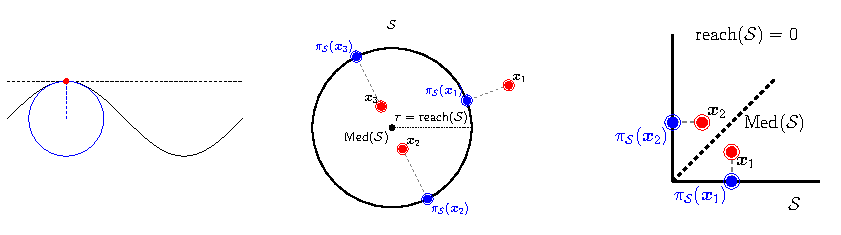
\includegraphics[width=\textwidth]{\toplevelprefix/chapters/appendixB/figs/curvature-fig.pdf}
%
%     \caption{Curvature and reach. \textbf{Left:} Abstractly, curvature can be
%     thought of as quantifying the deviation of a smooth surface from its local
%     linear approximation. For curves, there is a precise characterization of
%     this in terms of the ``radius of curvature'' of an associated circle.
%     \textbf{Center:} The reach defines curvature in terms of injectivity of the
%     projection function onto the set, allowing it to be defined independent of
%     differentiability. In the case of $\cS$ a circle, the medial axis is the
%     circle's center, and the reach is the circle's radius. \textbf{Right:} Sets
%     with zero reach have some form of defective regularity. For example,
%     `corners' induce zero reach.}
%     \label{fig:curvature-reach}
% \end{figure}
%
% \subsection{Geometric Regularity: Curvature and Reach}
%
% For a set with geometric structure that is sufficiently smooth (say
% differentiable), regularity can be understood in terms of \textit{curvature}:
% how rapidly the set deviates from its local linear approximation at a point
% (\Cref{fig:curvature-reach}, left). In
% a sense, this can be thought of analogously to the second-order Taylor
% approximation in the theory of functions of a real variable.
% The study of curvature is considerably deep, and carefully harnessing it has led
% to the resolution of some of the most longstanding open problems in mathematics
% (perhaps most famously, Perelman's proof of the Poincar\'{e} conjecture
% \cite{Perelman2002-bt,Perelman2003-xe,Perelman2003-yk}).
%
% We will impose a curvature condition on the support set $\cS$ slightly
% indirectly, using a quantity known as the \textit{reach} \cite{Federer1959-gk}.
% This will allow us to avoid explicit assumptions of smoothness on the set $\cS$,
% since the content of \Cref{thm:covering-number-rate-distortion} is phrased
% purely in terms of metric quantities.
% Our exposition of this property is influenced by the presentation of
% \textcite{Aamari2019-mp}. For a (closed) set $\cS \subset \R^D$, consider the
% distance function to the set: for any $\vx \in \R^D$,
% \begin{equation}\label{eq:dist-func}
%     \dist(\vx, \cS) = \inf_{\vx' \in \cS} \norm*{\vx - \vx'}_2.
% \end{equation}
% For a compact set $\cS$, Weierstrass's theorem implies that for any $\vx \in
% \R^D$, there is always some $\vx' \in \cS$ attaining the infimum in the distance
% function. The reach is defined in terms of those points at which the infimum is
% \textit{uniquely} attained. Define the medial axis of $\cS$ by
% \begin{equation}
%     \mathrm{Med}(\cS) = \set*{
%         \vx \in \R^D \given \exists \vx' \neq \vx'' \in \cS,
%         \norm*{\vx - \vx'}_2 = \norm*{\vx - \vx''}_2 = \dist(\vx, \cS)
%     },
% \end{equation}
% which is the set of points at which the infimum is non-uniquely attained.
% We define the reach as
% \begin{equation}
%     \mathrm{reach}(\cS) = \inf_{\vx \in \cS} \dist(\vx, \mathrm{Med}(\cS)).
% \end{equation}
% The medial axis can be empty (consider a convex set $\cS$), in which case the
% reach is $+\infty$. If it is nonempty, the reach is finite. It can be understood
% as a notion of curvature (\Cref{fig:curvature-reach}, center and right).
% We assume:
% \begin{assumption}\label{assumption:positive-reach}
%     The support $\cS \subset \R^D$ of the random variable $\vx$ is compact,
%     with positive reach.
% \end{assumption}
%
% The main consequence of \Cref{assumption:positive-reach} for our purposes is
% that the \textit{projection} onto the set $\cS$ can be uniquely defined for
% \textit{any} point below the reach. More precisely, if $\cS$ satisfies
% $\mathrm{reach}(\cS) = \tau > 0$, then for any $\vx$ with $\dist(\vx, \cS)
% < \tau$, the optimization problem
% \begin{equation}
%     \argmin_{\vx' \in \cS}\, \norm*{\vx - \vx'}_2
% \end{equation}
% has a unique solution (it is attained, by compactness), and hence we can define
% a projection mapping
% \begin{equation}
%     \pi_{\cS}(\vx) \doteq
%     \argmin_{\vx' \in \cS}\, \norm*{\vx - \vx'}_2
% \end{equation}
% on the domain $\set{\vx \in \R^D \given \dist(\vx, \cS) < \tau}$, with range
% $\cS$. This fact will be used in the proof of
% \Cref{thm:covering-number-rate-distortion}.
%
% To avoid excessive technical complications, we make an additional simplifying
% assumption on the support set $\cS$. To introduce it, we need two additional
% geometric definitions that are fundamental in the theory of sets of positive
% reach.
% Let $\mathrm{tan}(\cS, \vx)$ denote the tangent cone to $\cS$ at a point $\vx
% \in \cS$:
% \begin{equation}\label{eq:tangent-cone}
%     \mathrm{tan}(\cS, \vx) = \set*{\vu \in \R^D \mid \exists \vx_i \in \cS, r_i
%     > 0 \::\: r_i(\vx_i - \vx) \to_{i \to \infty} \vx} \cup \set{\Zero}.
% \end{equation}
% In differential geometry, the tangent space represents the best local linear
% approximation to an underlying manifold. In the theory of sets of positive
% reach, the previous definition gives a similar but more general structure which
% does not require differentiability.
% The normal cone to $\cS$ at $\vx \in \cS$ is defined in terms of the tangent
% cone:
% \begin{equation}\label{eq:normal-cone}
%     \mathrm{nor}(\cS, \vx) = \set*{\vu \in \R^D \mid \ip{\vu}{\vv} \leq 0,\,
%     \forall \vv \in \mathrm{tan}(\cS, \vx)}.
% \end{equation}
% In differential geometry, the normal space is the orthogonal complement of the
% tangent space---it gives the set of directions which (locally) move away from
% the manifold at a given point. The previous definition generalizes this notion
% to non-differentiable sets, for which we need to consider tangent cones rather
% than tangent vector spaces; for cones, the preceding definition is an
% appropriate generalization of the orthogonal complement, as all elements of the
% normal cone make at least a $90$ degree angle with all elements of the tangent
% cone.
%
% \begin{assumption}\label{assumption:no-boundary}
%     The support $\cS \subset \R^D$ of the random variable $\vx$ has Hausdorff
%     dimension $d$, and if $d \geq 1$, the set $\cS^{(d-1)} = \set*{\vx \in \cS
%     \given \dim(\mathrm{nor}(\cS, \vx)) \geq D-d+1}$ is empty.
% \end{assumption}
%
% \Cref{assumption:no-boundary} is technical, but can be intuitively thought of as
% requiring the support set $\cS$ to have empty boundary, when viewed as
% a submanifold of $\bR^D$. In particular, \Cref{assumption:no-boundary} is
% satisfied whenever $\cS$ is a differentiable manifold without boundary, because
% in this case the tangent spaces are all vector spaces of the same dimension.
% We do not discuss Hausdorff dimension here, except to mention that it can be
% thought of as a generalization of the dimension of a subspace or a manifold to
% arbitrary subsets of $\bR^D$---see, e.g., \cite{Evans1991-pp} for more details.



% \subsection{Proof of
% \texorpdfstring{\Cref{thm:covering-number-rate-distortion}}{Relationship
% Between Rate Distortion and Covering}}
\subsection{Proof of Relationship Between Rate Distortion and Covering}

We briefly sketch the proof, then proceed to establishing three fundamental
lemmas, then give the proof. The proof will depend on notions introduced in the
sketch below.

Obtaining an upper bound on the rate distortion function
\eqref{eqn:rate-distortion-general} is straightforward: by the rate
characterization (i.e., the rate distortion function is the minimum rate of
a code for $\vx$ with expected squared $\ell^2$ distortion $\epsilon$), upper
bounding $\cR_{\epsilon}(\x)$ only requires demonstrating one code for $\x$ that
achieves this target distortion, and any $\epsilon$-covering of $\Supp(\x)$
achieves this, with rate equal to the base-$2$ logarithm of the cardinality of
the covering.
The lower bound is more subtle. We make use of the Shannon lower bound,
discussed in \Cref{rem:slb}: working out the constants in \cite[\S III,
(22)]{Linder1994-ej} gives a more precise version of the result quoted in
\Cref{eq:slb} (in bits, of course): for any random variable $\vx$ with compact
support and a density, it holds
\begin{equation}\label{eq:slb-appendix-1}
    \cR_{\epsilon}(\x)
    \geq
    h(\x)
    - \log \volume(B_{\epsilon})
    +
    \log
    \left(
    \frac{
    	2
    }
    {
    	D \Gamma(D/2)
    }
    \left(
    \frac{
    	D
    }
    {
    	2e
    }
    \right)^{D/2}
    \right),
\end{equation}
with entropy (etc.) in nats in this expression.
The constant can be easily estimated using Stirling's approximation.
A quantitative form of Stirling's approximation which is often useful gives
for any $x > 0$ \cite{Jameson2015-hy}
\begin{equation}
    \Gamma(x) \leq \sqrt{2\pi} x^{x - 1/2} e^{-x} e^{1/(12x)}.
\end{equation}
We will apply this bound to $\Gamma(D/2)$ in \Cref{eq:slb-appendix-1}.
We get
% Since $D \geq 1$, we have $e^{1/(6D)} \leq e^{1/6}$, and
\begin{align}
    \log
    \left(
    \frac{
        2
    }
    {
        D \Gamma(D/2)
    }
    \left(
    \frac{
        D
    }
    {
        2e
    }
    \right)^{D/2}
    \right)
    &\geq
    -\frac{1}{6D}
    +
    \log\left(
        \frac{2}{D} 
        \left(
        \frac{
            D
        }
        {
            2e
        }
        \right)^{D/2}
        \cdot
        \sqrt{\frac{D}{4\pi}}
        \left(
        \frac{D}{2e}
        \right)^{-D/2}
    \right)
    \\
    &=
    -\frac{1}{6D}
    - \frac{1}{2}\log D\pi,\label{eq:slb-constant-est}
\end{align}
which we can take for the explicit value of the constant $C_D$ in \Cref{eq:slb}.
Summarizing the fully quantified Shannon lower bound (in bits):
\begin{equation}\label{eq:slb-appendix}
    \cR_{\epsilon}(\x)
    \geq
    h(\x)
    - \log_2 \volume(B_{\epsilon})
    % - \frac{1}{2} \log(D\pi) 
    - O(\log D).
\end{equation}

Now, the important constraint for our current purposes is that the Shannon lower
bound requires the random variable $\vx$ to have a density, which rules out many
low-dimensional distributions of interest.
But let us momentarily consider the situation when $\vx$ does admit a density.
The assumption that $\vx$ is uniformly distributed on its support is easily
formalized in this setting: for any Borel set $A \subset \cS$, we have
\begin{equation}
    \Pr[\vx \in A] = \int_{A} \frac{1}{\volume(\cS)} \odif \vx.
\end{equation}
Then the entropy $h(\vx)$ is just
\begin{equation}
    h(\vx) = \log_2 \volume(\cS).
\end{equation}
The proof then concludes with a lemma that relates the ratio $\volume(\cS)
/ \volume(B_{\epsilon})$ to the $\epsilon$-covering number of $\cS$ by
$\epsilon$ balls.
% More generally, in particular for low-dimensional distributions, we can give
% a rigorous definition of $\vx$ being uniformly distributed on its support in
% terms of \sdb{COMPLETE}


To extend the program above to degenerate distributions satisfying
\Cref{assumption:union-of-spheres},
our proof of the lower bound in \Cref{thm:covering-number-rate-distortion} will
leverage an approximation argument of the actual low-dimensional
distribution $\vx$ by ``nearby'' low-dimensional distributions which have
densities.
% We will moreover ensure that the approximating sequence is 
% We will use \Cref{assumption:positive-reach} to ensure that this approximation
% is possible, and that the ``convergence'' that occurs is sufficiently regular
% for us to estimate the rate distortion of $\vx$ in terms of that of the
% approximating distributions. 
We will then link the parameter introduced in
the approximating sequence to the distortion parameter $\epsilon$ in order to
obtain the desired conclusion in \Cref{thm:covering-number-rate-distortion}.


\begin{definition}\label{def:thickening-set}
    Let $\cS$ be a compact set.
    % satisfies \Cref{assumption:positive-reach}.
    For any $\delta > 0$, define the $\delta$-thickening of $\cS$, denoted
    $\cS_{\delta}$, by
    \begin{equation}
        \cS_{\delta} = \set*{\vxi \in \R^D \given \mathrm{dist}(\vxi, \cS) \leq
        \delta}.
    \end{equation}
\end{definition}
The distance function referenced in \Cref{def:thickening-set} is defined by
\begin{equation}\label{eq:dist-func}
    \dist(\vxi, \cS) = \inf_{\vxi' \in \cS} \norm*{\vxi - \vxi'}_2.
\end{equation}
For a compact set $\cS$, Weierstrass's theorem implies that for any $\vxi \in
\R^D$, there is always some $\vxi' \in \cS$ attaining the infimum in the distance
function. 
% \eqref{eq:dist-func}, 
% and its properties discussed subsequently. 
Compactness of $\cS_{\delta}$ follows readily from compactness of $\cS$, so
$\volume(\cS_{\delta})$ is finite for any $\delta > 0$. It is then possible to
make the following definition of a thickened random variable, specialized to
\Cref{assumption:union-of-spheres}.

% \begin{definition}\label{def:thickening-rv}
%     Let $\vx$ be a random variable such that $\Supp(\vx) = \cS$ is compact.
%     Define the thickened random variable $\vx_{\delta}$ as being uniformly
%     distributed on the set $\cS_{\delta}$ (\Cref{def:thickening-set}).
% \end{definition}

\begin{definition}\label{def:thickening-rv-uos}
    Let $\vx$ be a random variable such that $\Supp(\vx) = \cS$ is a union of
    $K$ hyperspheres, distributed as in \Cref{assumption:union-of-spheres}.
    Denote the support of each component of the mixture by $\cS_k$.
    Define the thickened random variable $\vx_{\delta}$ as the mixture of
    measures where each component measure is uniform on the thickened set
    $\cS_{k, \delta}$ (\Cref{def:thickening-set}), for $k \in [K]$, with mixing
    weights $\pi_k$.
\end{definition}


\begin{lemma}\label{lem:rate-distortion-lb-uos}
    Suppose the random variable $\vx$ satisfies
    \Cref{assumption:union-of-spheres}. Then if $0 < \delta < \tfrac{1}{2}$, the
    thickened random variable $\vx_{\delta}$ (\Cref{def:thickening-rv-uos})
    satisfies for any $\epsilon > 0$
    \begin{equation}
        R_{\delta + \epsilon}(\vx_{\delta})
        \leq
        R_{\epsilon}(\vx).
    \end{equation}
\end{lemma}

The proof of \Cref{lem:rate-distortion-lb-uos} is deferred to
\Cref{sec:app-rate-dist-deferred-proofs}.
Using \Cref{lem:rate-distortion-lb-uos}, the above program can be realized,
because the random variable $\vx_{\delta}$ has a density that is uniform with
respect to the Lebesgue measure.

\begin{proof}[(Proof of \Cref{thm:covering-number-rate-distortion})]
    The upper bound is readily shown. If $S$ is any $\epsilon$-cover of the
    support of $\vx$ with cardinality $\cN_{\epsilon}(\Supp(\vx))$, then consider the
    coding scheme assigning to each $\vxi \in \Supp(\vx)$ the reconstruction
    $\hat{\vxi} = \argmin_{\vxi' \in S}\, \norm{\vxi - \vxi'}_2$, with ties
    broken arbitrarily. Then ties occur with probability zero, and the fact that
    $S$ covers $\Supp(\vx)$ at scale $\epsilon$ guarantees distortion no larger
    than $\epsilon$; the rate of this scheme is $\log_2 \cN_{\epsilon}(\Supp(\vx))$.

    For the lower bound, let $0 < \delta < \tfrac{1}{2}$, and consider the
    thickened random variable $\vx_{\delta}$. By
    \Cref{lem:rate-distortion-lb-uos}, we have
    \begin{equation}
        R_{\delta + \epsilon}(\vx_{\delta})
        \leq
        R_{\epsilon}(\vx).
    \end{equation}
    Since $\vx_{\delta}$ has a Lebesgue density that is uniform, we can then
    apply the Shannon lower bound, in the form \eqref{eq:slb-appendix}, to get
    \begin{equation}\label{eq:slb-proof}
        % h(\x)
        \log_2 \volume(\Supp(\vx_{\delta}))
        - \log_2 \volume(B_{\delta + \epsilon})
        - O(\log D)
        \leq
        R_{\epsilon}(\vx).
        % R_{\sqrt{2(\delta^2 + \epsilon^2)}}(\vx_{\delta}).
    \end{equation}
    Finally, we need to lower bound the ratio
    \begin{equation}
        \frac{
            \volume(\Supp(\vx_{\delta}))
        }
        {
            \volume(B_{\delta + \epsilon})
        }
    \end{equation}
    in terms of the covering number.
    Since $\Supp(\vx_{\delta}) = \Supp(\vx) + B_{\delta}$, where $+$ here
    denotes the Minkowski sum, a standard application of volume bound arguments
    (see e.g.\ \cite[Proposition 4.2.12]{Vershynin2018-br}) gives
    \begin{equation}
        \volume(\Supp(\vx_{\delta}))
        \geq
        \cN_{2\delta}(\Supp(\vx))
        \volume(B_{\delta}).
    \end{equation}
    Hence
    \begin{align}
        \frac{
            \volume(\Supp(\vx_{\delta}))
        }
        {
            \volume(B_{\delta + \epsilon})
        }
        &\geq
        \cN_{2\delta}(\Supp(\vx))
        \frac{
            \volume(B_{\delta})
        }
        {
            \volume(B_{\delta + \epsilon})
        }
        \\
        &=
        \cN_{2\delta}(\Supp(\vx))
        \left(
            \frac{
                \delta
            } 
            {
                \delta + \epsilon
            }
        \right)^D.
    \end{align}
    Choosing $\delta = \epsilon / 2$ gives from the Shannon lower bound
    \eqref{eq:slb-proof} and the above estimates
    \begin{equation}
        \log_2 \cN_{\epsilon}(\Supp(\vx))
        - O(D)
        \leq
        R_{\epsilon}(\vx),
    \end{equation}
    as was to be shown.

\end{proof}



\subsection{Deferred Proofs}\label{sec:app-rate-dist-deferred-proofs}

\begin{proof}[(Proof of \Cref{lem:rate-distortion-lb-uos})]
    It suffices to show that any code for $\vx$ with expected squared distortion
    $\epsilon^2$ produces a code for $\vx_{\delta}$ with the same rate and
    distortion not much larger, for a suitable choice of $\delta$.
    So fix such a code for $\vx$, achieving rate $R$ and expected squared
    distortion $\epsilon^2$. We write $\hat{\vx}$ for the reconstructed random
    variable using this code, and $\mathrm{q} : \Supp(\vx) \to \Supp(\vx)$
    for the associated encoding-decoding mapping (i.e., $\hat{\vx}
    = \mathrm{q}(\vx)$).

    Now let $\cS_k$ denote the $k$-th hypersphere in the support of $\vx$.
    There is an orthonormal basis $\vU_{k} \in \R^{D \times d_k}$ such that
    $\Span(\cS_k) = \Span(\vU_k)$.
    The following orthogonal decomposition of the support set $\cS$
    will be used repeatedly throughout the proof. 
    We have
    \begin{align}
        \cS_{\delta} 
        &= \set{\vxi \in \R^D \given \exists k \in [K] \::\: \dist(\vxi,
        \cS_k) \leq \delta}
        \\
        &= \bigcup_{k \in [K]} \set{\vxi \in \R^D \given \dist(\vxi,
        \cS_k) \leq \delta}.
    \end{align}
    By orthogonal projection, for any $k \in [K]$ any $\vxi \in \R^D$ can be
    written as $\vxi = \vxi^{\|} + \vxi^{\perp}$, with $\vxi^{\|} \in \Span(\cS_k)$
    and $\ip{\vxi^{\|}}{\vxi^\perp} = 0$.
    Then for any $\vxi' \in \cS_k$, we have
    \begin{align}
        \norm*{\vxi - \vxi'}_2^2 
        = 
        \norm*{\vxi^{\|} + \vxi^{\perp} - \vxi'}_2^2
        &=
        \norm*{\vxi^{\|}}_2^2 + \norm*{\vxi^{\perp}}_2^2 + \norm*{\vxi'}_2^2
        - 2 \ip*{\vxi^{\|}}{\vxi'}
        \\
        &\geq
        \norm*{\vxi^{\|}}_2^2 + \norm*{\vxi'}_2^2
        - 2 \ip*{\vxi^{\|}}{\vxi'}
        \\
        &=
        \norm*{\vxi^{\|} - \vxi'}_2^2.
    \end{align}
    Further, it is known that for any nonzero $\vxi^{\|} \in \Span(\cS_k)$,
    \begin{equation}
        \inf_{\vxi' \in \cS_k}\,
        \norm*{\vxi^{\|} - \vxi'}_2^2
        =
        \norm*{\vxi^{\|} - \frac{\vxi^{\|}}{\norm{\vxi^{\|}}_2}}_2^2.
    \end{equation}
    If $\vxi^{\|}$ is zero, it is clear that the above distance is equal to $1$
    for every $\vxi' \in \cS_k$.
    Hence, if we define a projection mapping
    $\pi_{\cS_k}(\vxi)$
    by
    \begin{equation}
        \pi_{S_k}(\vxi) = \frac{\vU_k\vU_k^\top \vxi}{\norm{\vU_k^\top \vxi}_2}
    \end{equation}
    for any $\vxi \in \R^D$ with $\vU_k^\top \vxi \neq \mathbf{0}$, then 
    $\pi_{\cS_k}(\vxi) = \argmin_{\vxi' \in \cS_k}\norm*{\vxi' - \vxi}_2$.
    We choose $0 < \delta < 1$, so that the thickened set $\cS_{\delta}$
    contains no points $\vxi \in \R^D$ at which any of the projection maps
    $\pi_{\cS_k}$ is not well-defined.
    So the thickened set $\cS_{\delta}$ satisfies
    \begin{align}
        \cS_{\delta} 
        &= \bigcup_{k \in [K]} \set*{\vxi \in \R^D \given 
        \norm*{\vxi - \frac{\vU_k\vU_k^\top \vxi}{\norm{\vU_k^\top \vxi}_2}}_2
        \leq \delta}.
    \end{align}
    These distances can be rewritten in terms of the orthogonal decomposition as 
    \begin{align}
        \norm*{\vxi - \frac{\vU_k\vU_k^\top \vxi}{\norm{\vU_k^\top \vxi}_2}}_2^2
        &=
        \norm*{\vxi}_2^2 - 2 \norm{\vU_k^\top \vxi}_2 + 1
        \\
        &=
        \norm*{\vxi^{\|}}_2^2 
        + \norm*{\vxi^{\perp}}_2^2
        - 2 \norm{\vU_k^\top \vxi^{\|}}_2 + 1
        \\
        &=
        \norm*{\vxi^{\perp}}_2^2
        + \left( \norm*{\vxi^{\|}}_2 - 1 \right)^2.
        \label{eq:distance-to-hypersphere}
    \end{align}
    We are going to show next that every such $\vxi \in \cS_{\delta}$ can be
    uniquely associated to a projection onto a single subspace in the mixture,
    which will allow us to define a corresponding projection onto $\cS$.
    Given a $\vxi \in \cS_{\delta}$, by the above, we can find a subspace
    $\vU_k$ such that the orthogonal decomposition $\vxi = \vxi^{\|}_k
    + \vxi^{\perp}_k$ satisfies
    \begin{equation}
        \norm*{\vxi^{\perp}_k}_2^2
        + \left( \norm*{\vxi^{\|}_k}_2 - 1 \right)^2
        \leq
        \delta^2.
    \end{equation}
    Consider the decomposition $\vxi = \vxi_j^{\|} + \vxi_j^{\perp}$ for some $j
    \neq k$. We have
    \begin{align}
        \norm*{\vxi_j^{\|}}_2
        =
        \norm*{
            \vU_j \vU_j^\top \vxi 
        }_2
        &=
        \norm*{
            \vU_j \vU_j^\top( \vU_k \vU_k^\top \vxi + (\vI - \vU_k \vU_k^\top)
            \vxi )
        }_2
        \\
        &=
        \norm*{
            \vU_j \vU_j^\top (\vI - \vU_k \vU_k^\top) \vxi
        }_2
        \\
        &\leq
        \norm*{
            (\vI - \vU_k \vU_k^\top) \vxi
        }_2
        =
        \norm*{
            \vxi_k^{\perp}
        }_2
        \leq \delta,
    \end{align}
    where the second line uses the orthogonality assumption on the subspaces
    $\vU_k$, and the third uses the fact that orthogonal projections are
    nonexpansive.
    Hence, the $j$-th distance satisfies
    \begin{equation}
        \norm*{\vxi^{\perp}_j}_2^2
        + \left( \norm*{\vxi^{\|}_j}_2 - 1 \right)^2
        \geq
        (1 - \delta)^2.
    \end{equation}
    This implies that if $0 < \delta < 1/2$, every $\vxi \in \cS_{\delta}$ has
    a unique closest subspace in the mixture.
    Hence, under this condition, the following mapping $\pi_{\cS} : \cS_{\delta}
    \to \cS$ is well-defined:
    \begin{equation}
        \pi_{\cS}(\vxi) 
        =
        \pi_{\cS_{k_\star}}(\vxi),
        \enspace\text{where}\enspace
        k_{\star} = \argmin_{k \in [K]}\,
        \dist(\vxi, \cS_{k}).
    \end{equation}

    % By the same token, we have the optimality condition 
    % \begin{equation}
    %     \vxi = \pi_{\cS_k}(\vxi)
    %     \iff
    %     \vxi = \vU_k \vz
    %     \enspace \text{for some} \enspace
    %     \vz \in \R^{d_k} \::\: \norm{\vz}_2 = 1.
    % \end{equation}
    % Hence, for any $\vxi \in \cS_{\delta}$, we can write $\vxi = \vU_k \vz
    % + \veps$ for some $k \in [K]$, some $\norm{\vz}_2 = 1$ and some
    % $\norm{\veps}_2 \leq \delta$.
    %     Given the representation $\vxi = \vU_k \vz + \veps$, 
    % notice that
    % \begin{equation}
    %     \dist(\vxi, \cS_k) = 
    % \end{equation}
    %
    % This implies that it is impossible to have $\vxi \in \cS_{\delta}$ and $k \neq k'$ for which
    % $\pi_{\cS_k}(\vxi) = \vxi$ and 
    % $\pi_{\cS_{k'}}(\vxi) = \vxi$. For if this were true, we would have $\vU_k
    % \vz = \vU_{k'} \vz'$ for some unit norm $\vz, \vz'$ by the optimality
    % conditions, contradicting the assumed mutual orthogonality of the subspaces $\vU_k$.
    % In addition, it follows from the assumed conditions $\sum_{k\in [K]} d_k = D$
    % and mutual orthogonality of each $\vU_k$ that for any $\vxi \in \R^D$, there
    % is 

    Now, we define a code for $\vx_{\delta}$ by
    \begin{equation}
        \hat{\vx}_{\delta} = \mathrm{q}( \pi_{\cS}(\vx_{\delta}) ).
    \end{equation}
    Clearly this is associated to a rate-$R$ code for $\vx_{\delta}$, because it
    uses the encoding-decoding mappings from the rate-$R$ code for $\vx$. We
    have to show that it achieves small distortion.
    We calculate
    \begin{align}
        \bE\left[ \norm*{ \vx_{\delta} - \hat{\vx}_{\delta} }_2^2 \right]
        &=
        \bE\left[ \norm*{ \vx_{\delta} - \mathrm{q}(\pi_{\cS}(\vx_{\delta})) }_2^2 \right]
        \\
        &\leq
        \left(
        \bE\left[ \norm*{ \vx_{\delta} - \pi_{\cS}(\vx_{\delta}) }_2^2
        \right]^{1/2}
        + \bE\left[ \norm*{ \pi_{\cS}(\vx_{\delta})
        - \mathrm{q}(\pi_{\cS}(\vx_{\delta})) }_2^2 \right]^{1/2}
        \right)^2,\label{eq:distortion-decomposition}
    \end{align}
    where the inequality uses the Minkowski inequality.
    Now, by \Cref{def:thickening-set,def:thickening-rv-uos}, we have
    deterministically
    \begin{equation}
        \norm*{ \vx_{\delta} - \pi_{\cS}(\vx_{\delta}) }_2^2
        \leq \delta^2,
    \end{equation}
    so the expectation also satisfies this estimate.
    For the second term, it will suffice to characterize the density of the
    random variable $\pi_{\cS}(\vx_{\delta})$ as being sufficiently close to the
    density of $\vx$---which, as \Cref{assumption:union-of-spheres} implies, is
    a mixture of uniform distributions on each sub-sphere $\cS_k$.
    By the argument above, every point $\vxi \in \cS_{\delta}$ can be associated
    to one and only one subspace $\vU_k$, which means that the mixture
    components in the definition of $\cS_{\delta}$ (recall
    \Cref{def:thickening-rv-uos}) do not overlap. Hence, the density
    $\pi_{\cS}(\vx_{\delta})$ can be characterized by studying the effect of
    $\pi_{\cS_k}$ on the conditional random variable $\vx_{\delta}$, conditioned
    on being drawn from $\cS_{k, \delta}$. Denote this measure by $\mu_{k,
    \delta}$.
    We claim that the pushforward of this measure under $\pi_{\cS_k}$ is uniform on $\cS_k$.
    To see that this holds, we recall
    \Cref{eq:distance-to-hypersphere},
    which gives the characterization
    \begin{equation}
        \cS_{k, \delta} = \set*{
            \vxi^{\|} + \vxi^{\perp} 
            \given 
            \vxi^{\|} \in \Span(\vU_k),
            \vxi^{\perp} \in \Span(\vU_k)^\perp,
            \norm*{\vxi^{\perp}}_2^2
            + \left( \norm*{\vxi^{\|}}_2 - 1 \right)^2
            \leq
            \delta
        }.
    \end{equation}
    The conditional distribution in question is uniform on this set; we need to
    show that the projection $\pi_{\cS_k}$ applied to this conditional random
    variable yields a random variable that is uniform on $\cS_k$.
    With respect to these coordinates, we have seen that $\pi_{\cS_k}(\vxi^\|
    + \vxi^\perp) = \vxi^\| / \norm{\vxi^{\|}}_2$.
    Hence, for any $\vxi \in \cS_{k}$, we have that the preimage of $\vxi$ in
    $\cS_{k, \delta}$ under $\pi_{\cS_k}$ is 
    \begin{equation}
        \pi_{\cS_k}^{-1}(\vxi) = \set*{
            r\vxi + \vxi^\perp 
            \given
            r > 0,
            \vxi^{\perp} \in \Span(\vU_k)^\perp,
            \norm*{\vxi^{\perp}}_2^2
            + \left( r - 1 \right)^2
            \leq
            \delta
        }.
        \label{eq:fiber-of-uos}
    \end{equation}
    To show that $(\pi_{\cS_k})_{\sharp} \mu_{k, \delta}$ is uniform, we need to 
    decompose the integral of the uniform density on $\cS_{k, \delta}$ in a way
    that makes it clear that each of the fibers 
    $\pi_{\cS_k}^{-1}(\vxi)$ (for each $\vxi \in \cS_k$) ``contributes'' equally
    to the integral.\footnote{More rigorously, this corresponds to decomposing
    the uniform density on $\cS_{k, \delta}$ into a regular conditional density
    corresponding to $\vxi \in \cS_{k}$, and showing that the corresponding
    density on $\vxi$ is uniform. The proof makes it clear this is true.}
    We have by \Cref{def:thickening-rv-uos}
    \begin{equation}
        \volume(\cS_{k, \delta})
        = \iint_{\Span(\vU_k) \times \Span(\vU_k)^\perp} \mathbf{1}_{
            \norm*{\vxi^{\perp}}_2^2
            + \left( \norm*{\vxi^{\|}}_2 - 1 \right)^2
            \leq
            \delta
        }
        \odif \vxi^{\|} \odif \vxi^{\perp}.
    \end{equation}
    In particular, the integration over the orthogonal coordinates factors. 
    Let $\odif \vtheta^{d}$ denote the uniform (Haar) measure on the sphere of
    radius $1$ in $\R^d$. Converting the $\vxi^{\|}$ integral to polar
    coordinates, we have
    \begin{equation}
        \volume(\cS_{k, \delta})
        = \int_{[0, \infty)} \int_{\bS^{d_k-1}} \int_{\Span(\vU_k)^\perp} 
        r^{d_k-1}
        \mathbf{1}_{
            \norm*{\vxi^{\perp}}_2^2
            + \left( r - 1 \right)^2
            \leq
            \delta
        }
        \odif r \odif \vtheta^{d_k} \odif \vxi^{\perp}.
    \end{equation}
    Comparing to the fiber representation \eqref{eq:fiber-of-uos},
    we see that we need to ``integrate out'' over the $r$ and $\vxi^\perp$
    components of the preceding integral in order to verify that the pushforward
    is uniform.
    But this is evident, as the previous expression shows that the value of this
    integral is independent of $\vxi^\|$---or, equivalently in context, the
    value of the spherical component $\vtheta^{d_k}$.

    Thus it follows from the above argument that $\pi_{\cS}(\vx_{\delta})$ is
    uniform.
    Because the assumption on $\delta$ implies that the mixture components in
    the distribution of $\vx_{\delta}$ do not overlap, the mixing weights
    $\pi_k$ are also preserved in the image $\pi_{\cS}(\vx_{\delta})$, and in
    particular, the distribution of $\pi_{\cS}(\vx_{\delta})$ is equal to the
    distribution of $\vx$.
    Hence the second term in \Cref{eq:distortion-decomposition} satisfies
    \begin{equation}
        \bE\left[ \norm*{ \pi_{\cS}(\vx_{\delta}) - \mathrm{q}(\pi_{\cS}(\vx_{\delta})) }_2^2 \right]
        \right)
        =
        \bE\left[ \norm*{ \vx - \mathrm{q}(\vx) }_2^2 \right]
        \right)
        \leq
        \epsilon^2,
    \end{equation}
    because $\mathrm{q}$ is a distortion-$\epsilon$ code for $\vx$.

    We have thus shown that the hypothesized rate-$R$, (expected squared)
    distortion-$\epsilon^2$ code for $\vx$ produces a rate-$R$, (expected
    squared) distortion $\delta + \epsilon)$ code for $\vx_{\delta}$.
    This establishes that
    \begin{equation}
        R_{\delta + \epsilon}(\vx_{\delta})
        \leq
        R_{\epsilon}(\vx),
    \end{equation}
    as was to be shown.


    % Choose $0 < \delta < \mathrm{reach}(\cS)$, using
    % \Cref{assumption:positive-reach}, so that the projection mapping $\pi_{\cS}
    % : \cS_{\delta} \to \cS$ is well-defined for any such $\delta$.
    % Define the reconstruction $\hat{\vx}_{\delta}$ by
    % \begin{equation}
    %     \hat{\vx}_{\delta} = \mathrm{q}( \pi_{\cS}(\vx_{\delta}) ).
    % \end{equation}
    % Clearly this is associated to a rate-$R$ code for $\vx_{\delta}$, because it
    % uses the encoding-decoding mappings from the rate-$R$ code for $\vx$. We
    % have to show that it achieves small distortion.
    % We calculate
    % \begin{align}
    %     \bE\left[ \norm*{ \vx_{\delta} - \hat{\vx}_{\delta} }_2^2 \right]
    %     &=
    %     \bE\left[ \norm*{ \vx_{\delta} - \mathrm{q}(\pi_{\cS}(\vx_{\delta})) }_2^2 \right]
    %     \\
    %     &\leq
    %     2 \left(
    %     \bE\left[ \norm*{ \vx_{\delta} - \pi_{\cS}(\vx_{\delta}) }_2^2 \right]
    %     + \bE\left[ \norm*{ \pi_{\cS}(\vx_{\delta}) - \mathrm{q}(\pi_{\cS}(\vx_{\delta})) }_2^2 \right]
    %     \right),
    % \end{align}
    % where the inequality uses Cauchy-Schwarz and the triangle inequality.
    %
    % Now, by \Cref{def:thickening-set,def:thickening-rv}, we have
    % deterministically
    % \begin{equation}
    %     \norm*{ \vx_{\delta} - \pi_{\cS}(\vx_{\delta}) }_2^2
    %     \leq \delta^2,
    % \end{equation}
    % so the expectation also satisfies this estimate.
    %
    % For the second term, noting that $\pi_{\cS}(\vx_{\delta})$ induces
    % a distribution $\mu_{\delta}$ on $\cS$ via the pushforward construction, it
    % suffices to show that this induced distribution $\mu_{\delta}$ is
    % sufficiently close to $\mu$, the distribution of $\vx$, to exploit the fact
    % that $\mathrm{q}$ achieves distortion $\epsilon^2$ and bound this term.
    % The argument is technical, using properties of positive-reach subsets of
    % $\R^D$.
\end{proof}



% \begin{lemma}\label{lem:thickened-uniform-projected-near-uniform}
%     Let $\vx_{\delta}$ denote the $\delta$-thickening (\Cref{def:thickening-rv})
%     of a random variable $\vx$ satisfying
%     \Cref{assumption:no-boundary,assumption:positive-reach}, with
%     $\cS = \Supp(\vx)$ and 
%     $\delta < \mathrm{reach}(\cS)$.
%     Let $\pi_{\cS}$ denote the projection onto $\cS$, and let $\mu_{\delta}$
%     denote the pushforward of the distribution of $\vx_{\delta}$ under
%     $\pi_{\cS}$.
%     Then $\mu_{\delta}$ admits a density with respect to $\dim(\cS)$-dimensional
%     Hausdorff measure on $\cS$, which satisfies
%     \begin{equation}
%         \sdb{UNIFORMITY EST}
%     \end{equation}
%
% \end{lemma}
%
% \begin{proof}
%     We compute the density of $\pi_{\cS}(\vx_{\delta})$ analytically, using the
%     coarea formula and some structural properties of sets of positive reach
%     satisfying \Cref{assumption:no-boundary}. Then we estimate it in terms of
%     the reach using curvature estimates for sets of positive reach. 
%
%     First, we recall a fundamental decomposition lemma for sets of positive
%     reach, due to Federer \cite{Federer1959-gk}. It asserts that the mapping
%     $f : \mathrm{nor}(\cS) \times (0, \delta] \to (\cS_{\delta} \setminus \cS)$
%     defined by $f(\vxi, \vu, r) = \vxi + r \vu$ is bijective and bi-Lipschitz,
%     where $\mathrm{nor}(\cS) = \set*{(\vxi, \vu) \in \bR^D \times \bS^{D-1}
%     \given \vxi \in \cS, \vu \in \mathrm{nor}(\cS, \vxi), \norm{\vu}_2 = 1}$ is the unit
%     normal bundle of $\cS$ (recall the definition of the normal cone of $\cS$ at
%     $\vx$ from \Cref{eq:normal-cone}) \cite[Proposition 16]{Thale2008-sv}.
%     Furthermore, we can decompose the unit normal bundle $\mathrm{nor}(\cS)$ in
%     a useful way under \Cref{assumption:no-boundary}: \cite[Remark
%     4.15(4)]{Federer1959-gk} implies that under this assumption, the tangent
%     cone (recall \Cref{eq:tangent-cone}) at every point $\vxi \in \cS$ is
%     actually a vector space with dimension $d$, and as a consequence, the normal
%     cone at every point is also a vector space (in particular the orthogonal
%     complement of the tangent cone/space), with dimension $D-d$. In particular,
%     the unit normal bundle satisfies $\mathrm{nor}(\cS) = \cS \times
%     \bS^{D-d-1}$ \sdb{This is not true, only isomorphic which generally changes
%     from point to point...}.
%
%     Next, we note from the above decomposition that the map $f$ can be expressed
%     as $f : \cS \times \bS^{D - d - 1} \times (0, \delta] \to (\cS_{\delta}
%     \setminus \cS)$. For any $t \in (0, \delta]$, consider the level sets
%     $\cS(t) = \set{\vxi \in \R^D \mid \dist(\vxi, \cS) = t}$. Then $\cS(t) \subset
%     \cS_{\delta}$, and for each $\vxi' \in \cS(t)$, there is a unique $(\vxi,
%     \vu) \in \cS \times \bS^{D-d-1}$ such that $f(\vxi, \vu, t) = \vxi'$.
%     In particular, by the definition of the distance function and the reach,
%     this implies that $\pi_{\cS}(\vxi') = \vxi$.
%     Hence we can compute the density of $\pi_{\cS}(\vx_{\delta})$ by
%     decomposing the integral over the set $\cS_{\delta}$ into independent
%     components stipulated by the map $f$.
%
%     Intuitively, this decomposition suggests that the projected distribution is
%     exactly uniform, as the normal space at every point of $\vx$ is identical.
%     To show this rigorously, we note that the density $p_{\delta}(\vxi)$
%     associated to $\mu_{\delta}$ must satisfy
%     \begin{equation}
%         p_{\delta}(\vx) = \bP[ \pi_{\cS}(\vx_{\delta}) = \vxi ].
%     \end{equation}
%     By the above decomposition, we have
%     \begin{equation}
%         \bP[ \pi_{\cS}(\vx_{\delta}) = \vxi ]
%         =
%         \bP[ \dist(\vx_{\delta}, \vxi) \leq \delta ],
%     \end{equation}
%     as a point $\vxi' \in \cS_{\delta}$ satisfies $\pi_{\cS}(\vxi') = \vxi$ if
%     and only if $\vxi' = \vxi + \vu r$ for some $\vu \in \bS^{D-d-1}$ and some
%     $r \in (0, \delta]$, and $\vx_{\delta}$ is uniform on $\cS_{\delta}$.
%
%
%     Applying the Area Formula, as in \cite[\S 3.2]{Thale2008-sv},
%     we obtain by the above reductions
%     \begin{equation}
%         \cH^{D}(\cS_{\delta})
%         =
%         \iint_{\cS \times \bS^{D-d-1}}
%         % \mathbf{1}_{B}(\vxi)
%         \int_0^\delta
%         \abs{\det Df(\vxi, \vu, r)} \odif r \odif \cH^{D-d-1}(\vu)
%         \cH^{d}(\vxi).
%     \end{equation}
%     The density of $\pi_{\cS}(\vx_{\delta})$ can be extracted from this
%     expression, via introducing an indicator and rearranging:
%     \begin{equation}
%         \mu_{\delta}(B)
%         =
%         \frac{1}{
%             \cH^{D}(\cS_{\delta})
%         }
%         \iint_{\cS \times \bS^{D-d-1}}
%         % \int_{\bS^{D-d-1}}
%         \mathbf{1}_{B}(\vxi)
%         \int_0^\delta
%         \abs{\det Df(\vxi, \vu, r)} \odif r \odif \cH^{D-d-1}(\vu)
%         \cH^{d}(\vxi),
%     \end{equation}
%     where $B \subset \cS$ is a Borel set of $\R^D$,
%     which implies the density $p_{\delta}(\vxi)$ at $\vxi \in \cS$ is
%     \begin{equation}\label{eq:density-expression-mudelta}
%         p_{\delta}(\vxi)
%         =
%         \frac{1}{
%             \cH^{D}(\cS_{\delta})
%         }
%         \int_{\bS^{D-d-1}}
%         \int_0^\delta
%         \abs{\det Df(\vxi, \vu, r)} \odif r \odif \cH^{D-d-1}(\vu).
%     \end{equation}
%     To prove the result, we will obtain upper and lower bounds on this
%     expression in terms of the reach. 
%     We calculate the (image of an arbitrary vector of the) Jacobian of $f$ at
%     a point as
%     \begin{equation}
%         Df(\vxi, \vu, r)(\Delta \vxi, \Delta \vu, \Delta r)
%         = \Delta \vxi + \vu \Delta r + r \Delta \vu.
%     \end{equation}
%     For the Jacobian determinant in the above integral, it suffices to represent
%     the Jacobian in an orthonormal basis for the tangent space of $\cS \times
%     \bS^{D-d-1} \times (0, \delta]$ at an arbitrary $(\vxi, \vu, r)$ pair.
%     Following \cite[p. 563]{Zahle1986-cp} and \cite[p.\ 138]{Thale2008-sv}, there is an 
%     orthonormal system $\vb_i(\vxi, \vu)$, $i = 1, \dots, D-1$, with
%     corresponding principal curvatures $\kappa_i(\vxi, \vu) > 0$, such that each
%     $\vb_i(\vxi, \vu)$ is orthogonal to $\vu$, and the system
%     \begin{equation}
%         \va_i(\vxi, \vu) = \left(
%         \frac{1}{\sqrt{1 + \kappa_i^2(\vxi, \vu)}} \vb_i(\vxi, \vu),
%         \frac{\kappa_i(\vxi, \vu)}{\sqrt{1 + \kappa_i^2(\vxi, \vu)}} \vb_i(\vxi, \vu)
%         \right)_{i=1}^{D-1}
%     \end{equation}
%     is an orthonormal system for the tangent bundle of $\cS \times \bS^{D-d-1}$.
%     Representing the Jacobian in this basis gives
%     \begin{equation*}
%         Df(\vxi, \vu, r)(\va_i(\vxi, \vu), 0)
%         =
%         \frac{1+r\kappa_i(\vxi, \vu)}{\sqrt{1+\kappa_i^2(\vxi,\vu)}} \vb_i(\vxi,
%         \vu),
%     \end{equation*}
%     and $Df(\vxi, \vu, r)(\Zero, 1) = \vu$, so defining $\vB(\vxi, \vu) \in
%     \R^{D \times (D-1)}$ as the matrix with columns $\vb_i(\vxi, \vu)$ and
%     $\vD(\vxi,\vu)
%     \in \R^{(D-1)\times (D-1)}$
%     as the diagonal matrix with $i$-th diagonal entry
%     $(1+r\kappa_i(\vxi,\vu))/\sqrt{1+\kappa_i^2(\vxi,\vu)}$,
%     computing the Jacobian determinant is equivalent to computing the
%     square root of the determinant of
%     \begin{equation}
%         \begin{bmatrix}
%             \vB\vD & \vu
%         \end{bmatrix}
%         \begin{bmatrix}
%             \vB\vD & \vu
%         \end{bmatrix}^\top.
%     \end{equation}
%     Here, we note that $[\vB, \vu]$ is an orthonormal matrix by construction. So
%     the determinant is just the determinant of $\abs{\vD}$.
%     In particular, we have shown
%     \begin{equation}\label{eq:jacobian-determinant-reach}
%         \abs{ \det Df(\vxi, \vu, r)}
%         =
%         \prod_{i=1}^{D-1}
%         \abs{1+r\kappa_i(\vxi,\vu)}/\sqrt{1+\kappa_i^2(\vxi,\vu)}.
%     \end{equation}
%
%     We finally estimate these principal curvatures using their definition in
%     \cite{Zahle1986-cp}. They can be related to the principal curvatures of the
%     hypersurface $\cS(r)$ for any $r \in (0, \delta]$, which by
%     \cite{Federer1959-gk} is a $C^1$ manifold with Lipschitz outer normal
%     $\nu_r : \cS(r) \to \bS^{D-1}$, and therefore has principal curvatures
%     $\kappa_i^r(\vxi + r \vu )$
%     defined almost everywhere as the eigenvalues of the self-adjoint operator $D
%     \nu_r(\vy)$ for $\vy = \vxi + r \vu$.
%     These can be related to the principal curvatures defined above by (see
%     \cite{Zahle1986-cp})
%     \begin{equation}\label{eq:principal-curvatures}
%         \kappa_i^r(\vxi + r \vu ) = \frac{\kappa_i(\vxi, \vu)}{1
%         + r \kappa_i(\vxi, \vu)}.
%     \end{equation}
%     \textit{A priori} the eigenvalues $\kappa_i^r(\vxi + r \vu )$ are arbitrary
%     real numbers, but the previous formula implies a constraint: in order for  
%     \eqref{eq:principal-curvatures} to be well-defined for every $0
%     < r \leq \delta < \mathrm{reach}(\cS)$, the denominator must not vanish for
%     such $r$. If $\kappa_i(\vxi, \vu) < 0$, this demands that $1
%     + r \kappa_i(\vxi, \vu) > 0$ for all such $r$; equivalently
%     \begin{equation}
%         \kappa_i(\vxi, \vu) > -\frac{1}{r}.
%     \end{equation}
%     Because the LHS of this bound does not depend on $r$, this implies
%     by taking a supremum over $\delta < \mathrm{reach}(\cS)$
%     \begin{equation}\label{eq:principal-curvatures-not-too-neg}
%         \kappa_i(\vxi, \vu) > -\frac{1}{\mathrm{reach}(\cS)}.
%     \end{equation}
%     It is also clear that $\kappa_i(\vxi, \vu) = +\infty$ is possible, in which
%     case \eqref{eq:jacobian-determinant-reach} is interpreted in a limiting
%     sense.
%     
%     \sdb{This graf is not right, we can get them to have magnitude equal to this
%     though? The sign depends on $\vu$? (or the sign is always negative...? it
%     depends on normal outward or inward...)}
%     In addition, in our setting where these principal curvatures are associated to the level
%     sets $\cS(r)$, we have a simplification, using the fact (as
%     established above using the map $f$) that $\cS(r) = \cS \times r\bS^{D-d-1}$.
%     This shows in particular that the tangent space at any point of $\cS(r)$,
%     expressed as $\vxi + r \vu$ by the decomposition above,
%     factors into a direct sum of the tangent space to $\cS$ at $\vxi$ and the
%     tangent space to $r\bS^{D-d-1}$ at $r \vu$, which does not depend on $r$.
%     Because the sphere is a homogeneous space, its principal curvatures do not
%     depend on $\vu$ (e.g., \cite{Lee2018-xb}); following the remark of
%     \textcite[\S 1]{Zahle1986-cp}, we compute these $D-d-1$ principal curvatures
%     $\kappa_i^r(\vxi + r \vu)$ as $1/r$, uniformly in $\vxi$ and $\vu$. It then
%     follows that the associated limit principal curvatures satisfy
%     $\kappa_i(\vxi, \vu) = +\infty$, so if we assume these are sorted in
%     ascending order, we can express \eqref{eq:jacobian-determinant-reach}
%     as
%     \begin{equation}\label{eq:jacobian-determinant-reach-lowdim}
%         \abs{ \det Df(\vxi, \vu, r)}
%         =
%         r^{D-d-1}
%         \prod_{i=1}^{d}
%         \abs{1+r\kappa_i(\vxi,\vu)}/\sqrt{1+\kappa_i^2(\vxi,\vu)}.
%     \end{equation}
%
%     Now we estimate \eqref{eq:jacobian-determinant-reach-lowdim} using
%     \eqref{eq:principal-curvatures-not-too-neg}.
%     For $r>0$, the function $g(x) = (1 + rx)^2 / (1 + x^2)$ has (by calculus)
%     two critical points at $x=r$ and $x=-1/r$; inspection shows that the
%     critical point at $x=-1/r$ is a minimum, and at $x=r$, a maximum, since the
%     values here satisfy $g(r) = 1 + r^2$ and $g(-1/r) = 0$, and moreover
%     $g(+\infty) = g(-\infty) = r^2$.
%     In addition, the function $g$ is monotone increasing from $x=-1/r$ to
%     $x=r$.
%     We apply this to \eqref{eq:jacobian-determinant-reach-lowdim}, where the principal
%     curvatures are playing the role of $x$; using
%     \eqref{eq:principal-curvatures-not-too-neg}, we have for all $i \in [d]$, $\vxi$,
%     $\vu$ if $r < \mathrm{reach}(\cS)$ 
%     \begin{equation}
%         \frac{{\mathrm{reach}(\cS) - r}}{\sqrt{1 + \mathrm{reach}(\cS)^2}}
%         \leq
%         \abs{1+r\kappa_i(\vxi,\vu)}/\sqrt{1+\kappa_i^2(\vxi,\vu)}
%         \leq
%         \sqrt{1 + r^2}.
%     \end{equation}
%
%     % Similarly, we can improve the lower bound.
%     % By the above, the function $g$ is monotone increasing from $x=-1/r$ to
%     % $x=r$, and monotone decreasing for $x \geq r$. So, if $x \geq -1/2r$, we
%     % have $g(x) \geq r^2 / (1 + 4r^2)$.
%     % In particular, if $r < \mathrm{reach}(\cS) / 2$, 
%     % the above bound can be improved to
%     % \begin{equation}
%     %     \frac{r}{\sqrt{1 + 4r^2}}
%     %     <
%     %     \abs{1+r\kappa_i(\vxi,\vu)}/\sqrt{1+\kappa_i^2(\vxi,\vu)}
%     %     \leq
%     %     \sqrt{1 + r^2},
%     % \end{equation}
%     % which can be relaxed using subadditivity of the square root to 
%     % \begin{equation}
%     %     \frac{r}{1 + 2r}
%     %     <
%     %     \abs{1+r\kappa_i(\vxi,\vu)}/\sqrt{1+\kappa_i^2(\vxi,\vu)}
%     %     \leq
%     %     1 + r.
%     % \end{equation}
%
%     Thus, we have the Jacobian determinant estimates (via \eqref{eq:jacobian-determinant-reach})
%     \begin{equation}
%         \frac{r^{D-1}}{(1 + 2r)^{D-1}}
%         \leq
%         \abs{ \det Df(\vxi, \vu, r)}
%         \leq
%         (1 + r)^{D-1}.
%     \end{equation}
%     Hence, we can estimate the density of $\mu_{\delta}$, denoted
%     $p_{\delta}(\vxi)$, via \eqref{eq:density-expression-mudelta} as 
%     \begin{equation}
%         \int_{\bS^{D-d-1}}
%         \int_0^\delta
%         \left( \frac{r}{1 + 2r}\right)^{D-1}
%         \odif r \odif \cH^{D-d-1}(\vu)
%         \leq
%         \cH^{D}(\cS_{\delta})
%         p_{\delta}(\vxi)
%         \leq
%         \int_{\bS^{D-d-1}}
%         \int_0^\delta
%         (1 + r)^{D-1}
%         \odif r \odif \cH^{D-d-1}(\vu)
%     \end{equation}
%     whenever $ r < \mathrm{reach}(\cS) / 2$, here implied by $\delta
%     < \mathrm{reach}(\cS)/2$.
%     The integrals on both sides of this bound can be factored into independent
%     integrals over $r$ and $\vu$. We get
%     \begin{equation}
%         \int_0^\delta
%         \left( \frac{r}{1 + 2r}\right)^{D-1}
%         \odif r
%         \leq
%         \frac{
%             \cH^{D}(\cS_{\delta})
%             p_{\delta}(\vxi)
%         }{
%             \volume(\bS^{D-d-1})
%         }
%         \leq
%         \int_0^\delta
%         (1 + r)^{D-1}
%         \odif r,
%     \end{equation}
%     whence
%     \begin{equation}
%         \int_0^\delta
%         \left( \frac{r}{1 + 2r}\right)^{D-1}
%         \odif r
%         \leq
%         \frac{
%             \cH^{D}(\cS_{\delta})
%             p_{\delta}(\vxi)
%         }{
%             \volume(\bS^{D-d-1})
%         }
%         \leq
%         \frac{1}{D} \left[
%             (1 + \delta)^D - 1
%         \right]
%     \end{equation}
%
%
%
%
%
%
%
%
%
%
%
% \end{proof}
%
% \begin{remark}
%     The conclusion of \Cref{lem:thickened-uniform-projected-near-uniform} has
%     a poor (exponential) dependence on the dimension $D$. This is due to needing
%     to treat possible negative curvature with worst-case estimates, as the proof
%     shows. Studying the proof demonstrates that if one adds the assumption that
%     all the principal curvatures are nonnegative, a lower bound for the density
%     of the projected thickened random variable can be derived that matches the
%     upper bound, greatly improving the obtained rate.
%
%     It is also likely that the exponential rate, which depends on $D$, can be
%     improved to $d$, the Hausdorff dimension of the support set $\cS$, with
%     a more refined analysis of the principal curvatures of the thickened
%     supports $\cS(t)$, $0 < t \leq \delta < \mathrm{reach}(\cS)$, given that
%     these are generated by thickening a $d$-dimensional set.
% \end{remark}








\end{document}
